\chapter{ State of the art theory}
\chaptertoc{}
%
\linenumbers

%
\section{Introduction to the many-body problem} \label{sec:BO_approx}
In this thesis, most of the computed quantities are not based on any parameter. The only input required is the chemical composition of the system, \textit{i.e.} the atomic numbers of the atoms constituting the crystal. This way of calculation is called \textit{ab initio}. It is a powerful framework since it does not require to fit any parameter to experiments and it can include all the physical phenomena one wants to consider. One of the shortcomings is that we often need to resort to approximations for the problems to be solvable numerically.
To perform such calculations, we need to consider all nuclei and all electrons in the crystal, as well as all the interactions between them. The system of interacting electrons and nuclei in a material can be described by the following Hamiltonian :
\begin{align}
	\hat{H} = &- \sum_I \frac{\hbar^2}{2 M_I} \nabla^2_I + \frac{1}{2} \sum_{I\neq J} \frac{Z_I Z_J e^2}{\left| \RR_I - \RR_J \right|} \nonumber \\
	&- \frac{\hbar^2}{2m_e} \sum_i \nabla^2_i + \frac{1}{2} \sum_{i\neq j} \frac{e^2}{\left| \rr_i - \rr_j \right|} - \sum_{i,I} \frac{Z_I e^2}{\left|\rr_i - \RR_I \right|}
\end{align}
where capital indices refer to nuclei and lowercase indices refer to electrons. $Z_I$, $M_I$ and $\RR_I$ are the atomic number, the mass and the position in real space of nucleus $I$, and $m_e,\rr_i$ are the electron mass and the electron position in real space. In this thesis, unless explicitly specified, we will use the atomic units, that is $\hbar = m_e = e =\pi/\varepsilon_0 =1$.
The terms on the first line are the kinetic energy of the ions and the ion-ion interaction, respectively. On the second line we have the kinetic energy of electrons, that we will later denote $T_{ee}$, the electron-electron interaction $V_{ee}$ and finally the electron-nucleus interaction, which we will refer to as the external potential felt by electrons in equilibrium, $V_{ext}$. This Hamiltonian is difficult to solve for a system containing two nuclei and two electrons, and is untractable for a larger number of particles. The kinetic terms and the interaction terms can be solved separately, but their combination is a formidable problem.
To greatly simplify this Hamiltonian, we use the so-called Born-Oppenheimer approximation. It consists in considering that the nuclei move in a much longer time-scale than the electrons, because their masses are much greater than those of the electrons. Every time we compute the electronic part, we consider that the nuclei do not have time to move from their equilibrium position. \cite{monserrat2018electron} We can then split the Hamiltonian into a nuclear term and an electronic term, and the nuclear part is just an additive constant. The electronic Hamiltonian then reads :
\be
	\hat{H} = \hat{T_e} + \hat{V}_{ee} + \hat{V}_{ext}
\ee
The first and second term are universal for all systems.The peculiarities of any systems are included in the last term in the above equation.

\section{Density Functional Theory}
\acrfull{DFT} is vastly used in solid-state physics and quantum chemistry. In this thesis, it will be the starting tool to compute structural and electronic properties of our systems. The idea behind \acrshort{DFT} is to replace the real system of interacting electrons by an auxiliary system of non-interacting particles evolving in an effective potential. \acrshort{DFT} is an exact theory in principle and allows one to compute the ground state of the many-electron system.

\acrshort{DFT} is based on the work of Hohenberg and Kohn who stated and proved two fundamental theorems. \cite{hohenberg1964} The first one ensures there is a one-to-one correspondence between the electronic density and the external potential acting on the system. The second theorem states that the total energy of the system is a functional of the electronic density.
The total energy of a system of interacting electrons is written as :
\be
	E = \expval{\hat{H}}{\Psi} = \expval{\hat{T} + \hat{V}_{ee} }{\Psi} + \int d\rr v_{ext}(\rr)n(\rr)
\ee
By virtue of the Hohenberg and Kohn theorems, the total energy is a functional of the density and can be written as :
\be
 	E_{HK}[n] = F_{HK}[n] + \int d\rr v_{ext}(\rr)n(\rr)
	\label{eq:E_HK}
\ee
where $F_{HK}[n] = \la \hat{T} \ra + \la \hat{V}_{ee} \ra$ is a universal functional of the density, \emph{ie} the dependence on $n$ of the functional is the same for all systems. The ground-state energy $E = E_0$ is the minimum of the energy functional at the ground-state density $n=n_0$. To be able to compute these quantities, Kohn and Sham reformulated the problem into an auxiliary system of non-interacting particles, that has the same density as the real system.\cite{kohn1965} Its energy is :
\begin{equation}
	E_{ip}[n] = T_{ip}[n] + \int d\rr v_{\text{eff}}(\rr)n(\rr)
\end{equation}	
The total wavefunction of the system is expressed as a Slater determinant of single-particle wavefunctions : $\ket{\Psi} =\ket{\psi_1\psi_2 \ldots \psi_{N_e}}$. This reformulation is particularly helpful because it allows the kinetic energy term to be calculated analytically :
\begin{equation}
	T_{ip} =  \sum_i^{N_e} \bra{\psi_i}-\frac{\nabla_i}{2} \ket{\psi_i}
\end{equation}
The expression for the total energy functional in Eq. \eqref{eq:E_HK} can be rewritten as :
\be
	E_{KS}[n] = T_{ip}[n] + \int d\rr v_{ext}(\rr)n(\rr) + E_H[n] + E_{xc}[n]
\ee
where $T_{ip}$ is the kinetic energy of the independent particles with density $n$, $E_H$ is the Hartree energy, which is the classical electrostatic interaction :
\be
	E_H[n] = \int d\rr d\rr' \frac{n(\rr')n(\rr)}{\left|\rr - \rr' \right|}
	\label{eq:E_Hartree}
\ee
and $E_{xc}$ is the exchange-correlation energy functional defined as :
\be
	E_{xc}[n] = \langle \hat{T} \rangle - T_{ip}[n] + \langle \hat{V}_{ee} \rangle - E_H[n].
\ee
It is the difference between the exact kinetic energy and the independent particle one, $T_{ip}$, plus the difference between the exact electron-electron interaction and the Hartree energy functional. Hence it contains the quantum effects of exchange and correlation of fermions.

Since the auxiliary system is an ensemble of independent particles, one can write the so-called Kohn-Sham equations for each individual particle $i$ :
\be
 	\( -\frac{\nabla^2}{2} + v_{\text{eff}}(\rr)\) \psi_i(\rr) = \epsilon_i \psi_i(\rr). \label{eq:KS_eqs}
\ee
They are analogous to Schrödinger equation for a particle evolving in a local effective potential $v_{\text{eff}}$, that we have yet to determine. Their solutions are the auxiliary system's eigenvalues $\epsilon_i$ and eigenvectors $\psi_i$. Use these eigenfunctions we can construct the electronic density as  :
\begin{equation}
 	n(\rr) = \sum_i f_i \left| \psi_i\right|^2 \label{eq:DFT_n_vs_psi}
\end{equation}
where $f_i$ is the occupation number of state $i$. 
Applying the variational principle to $E_{ip}$ and $E_{KS}$ we get 
\begin{align}
    \frac{\delta E_{ip}[n]}{\delta n} \Biggr|_{n_0} = 0 &\implies \frac{\delta T_{ip}[n]}{\delta n} \Biggr|_{n_0} = - v_{\text{eff}}(\rr) \\
    \frac{\delta E_{KS}[n]}{\delta n} \Biggr|_{n_0} = 0 &\implies \frac{\delta T_{ip}[n]}{\delta n} \Biggr|_{n_0} = - v_H(\rr) - \frac{\delta E_{xc}[n]}{\delta n} \Biggr|_{n_0} - v_{ext}(\rr)
\end{align}
Using the fact that the total kinetic energy is independent of the density at fixed number of particles, we get :
\begin{align}
\begin{split}
	v_{\text{eff}}(\rr) &= v_{ext}(\rr) + \frac{\delta E_H[n]}{\delta n(\rr)} + \frac{\delta E_{xc}[n]}{\delta n(\rr)} \\
	&\equiv v_{ext}(\rr) + v_H([n],\rr) + v_{xc}([n],\rr). \label{eq:KS_potential}
\end{split}
\end{align}
At this point, we see that we have to solve the many-electron problem self-consistently. Indeed, the density is obtained by solving the Kohn-Sham equations which contain the effective potential. In turn, this potential depends on the density. In practice, one starts from a guess density and iterate over the self-consistent cycle until the quantities of interest vary less than an arbitrary threshold. \\
Density Functional Theory is often used as a reference for bandgaps and electronic dispersion calculations. One has to be careful when interpreting Kohn-Sham eigenvalues, because they do not bear any physical meaning. First, there is no guarantee that one can find an auxiliary system of non-interacting particles for any real system. Then, the excited states and bandgaps are not the physical ones.\cite{fiolhais2003primer} This is why we will use a more refined theory presented in the next section.

Up to now, \acrshort{DFT} is in principle an exact theory, as long as one can define an auxiliary system with the same density as the real system. However, there exists no analytical form of the exchange-correlation potential. Hence we will then have to resort to approximations to compute the density in practice.

\subsubsection{Exchange-correlation functional approximations}
The \textbf{\acrfull{LDA}} is the first one that we present, and that we used for most of the results in this thesis. It was proposed by Kohn and Sham.\cite{kohn1965} It consists in replacing the exchange-correlation energy density by the one of the homogeneous electron gas, which is local in the density :
\be
	E_{XC}^{LDA} [n] = \int d\rr \ \epsilon^{HEG}_{xc}(n(\rr))
\ee
The exchange energy density of the homogeneous electron gas is known : $\epsilon_X^{HEG}(n) = -\tfrac{3}{4}(\tfrac{3}{\pi}n)^{(1/3)}$, and the correlation energy density is obtained from interpolation of an accurate quantum Monte Carlo simulation for various values of densities.\cite{ceperley1980ground} The LDA is relatively simple and computationally inexpensive. It gives a satisfactory description of system with slowly-varying density, but also surprisingly good results for a larger range of materials. For instance, for layered materials such as hBN, the interlayer binding energies are rather accurate, due to the tendency of overbinding of the LDA which cancels the error induced by the lack of van der Waals interactions.

In the \textbf{\acrfull{GGA}} the exchange-correlation energy density contains an additional dependence in the gradient of the density :
\be
 	E_{XC}^{GGA} [n] = \int d\rr \ \epsilon^{GGA}_{xc}(n(\rr),\nabla n(\rr)).
\ee
This type of functional is obtained by setting some parameters to satisfy exact constraints. The structural and bonding properties are often improved with respect to the \acrshort{LDA}.
There are many more approximations going beyond LDA and GGA functionals that we will not detail here,\cite{martin2020electronic} as we did not use them for the DFT calculations in this thesis.
%

\subsubsection{Pseudopotentials}
In our work it is not necessary to describe every single electron in the crystal. In fact, for the range of energies we are interested in, the electrons that can be optically excited are those that occupy the highest valence shells.
The core electrons of the first $s$ and $p$ shells are bound too strongly to the nuclei to be excited by a few electron-Volts incoming light. Hence, to simplify the system, we use pseudopotentials to avoid describing the core electrons. Pseudopotentials solve the problem of the divergence of the Coulomb potential as $\rr \to 0$, which leads to rapid oscillations in the wave functions of the occupied orbitals.\cite{martin2020electronic}
\begin{figure}[h!tbp]
	\vspace{0.5cm}
	\setcapindent{2em}
	\centering
	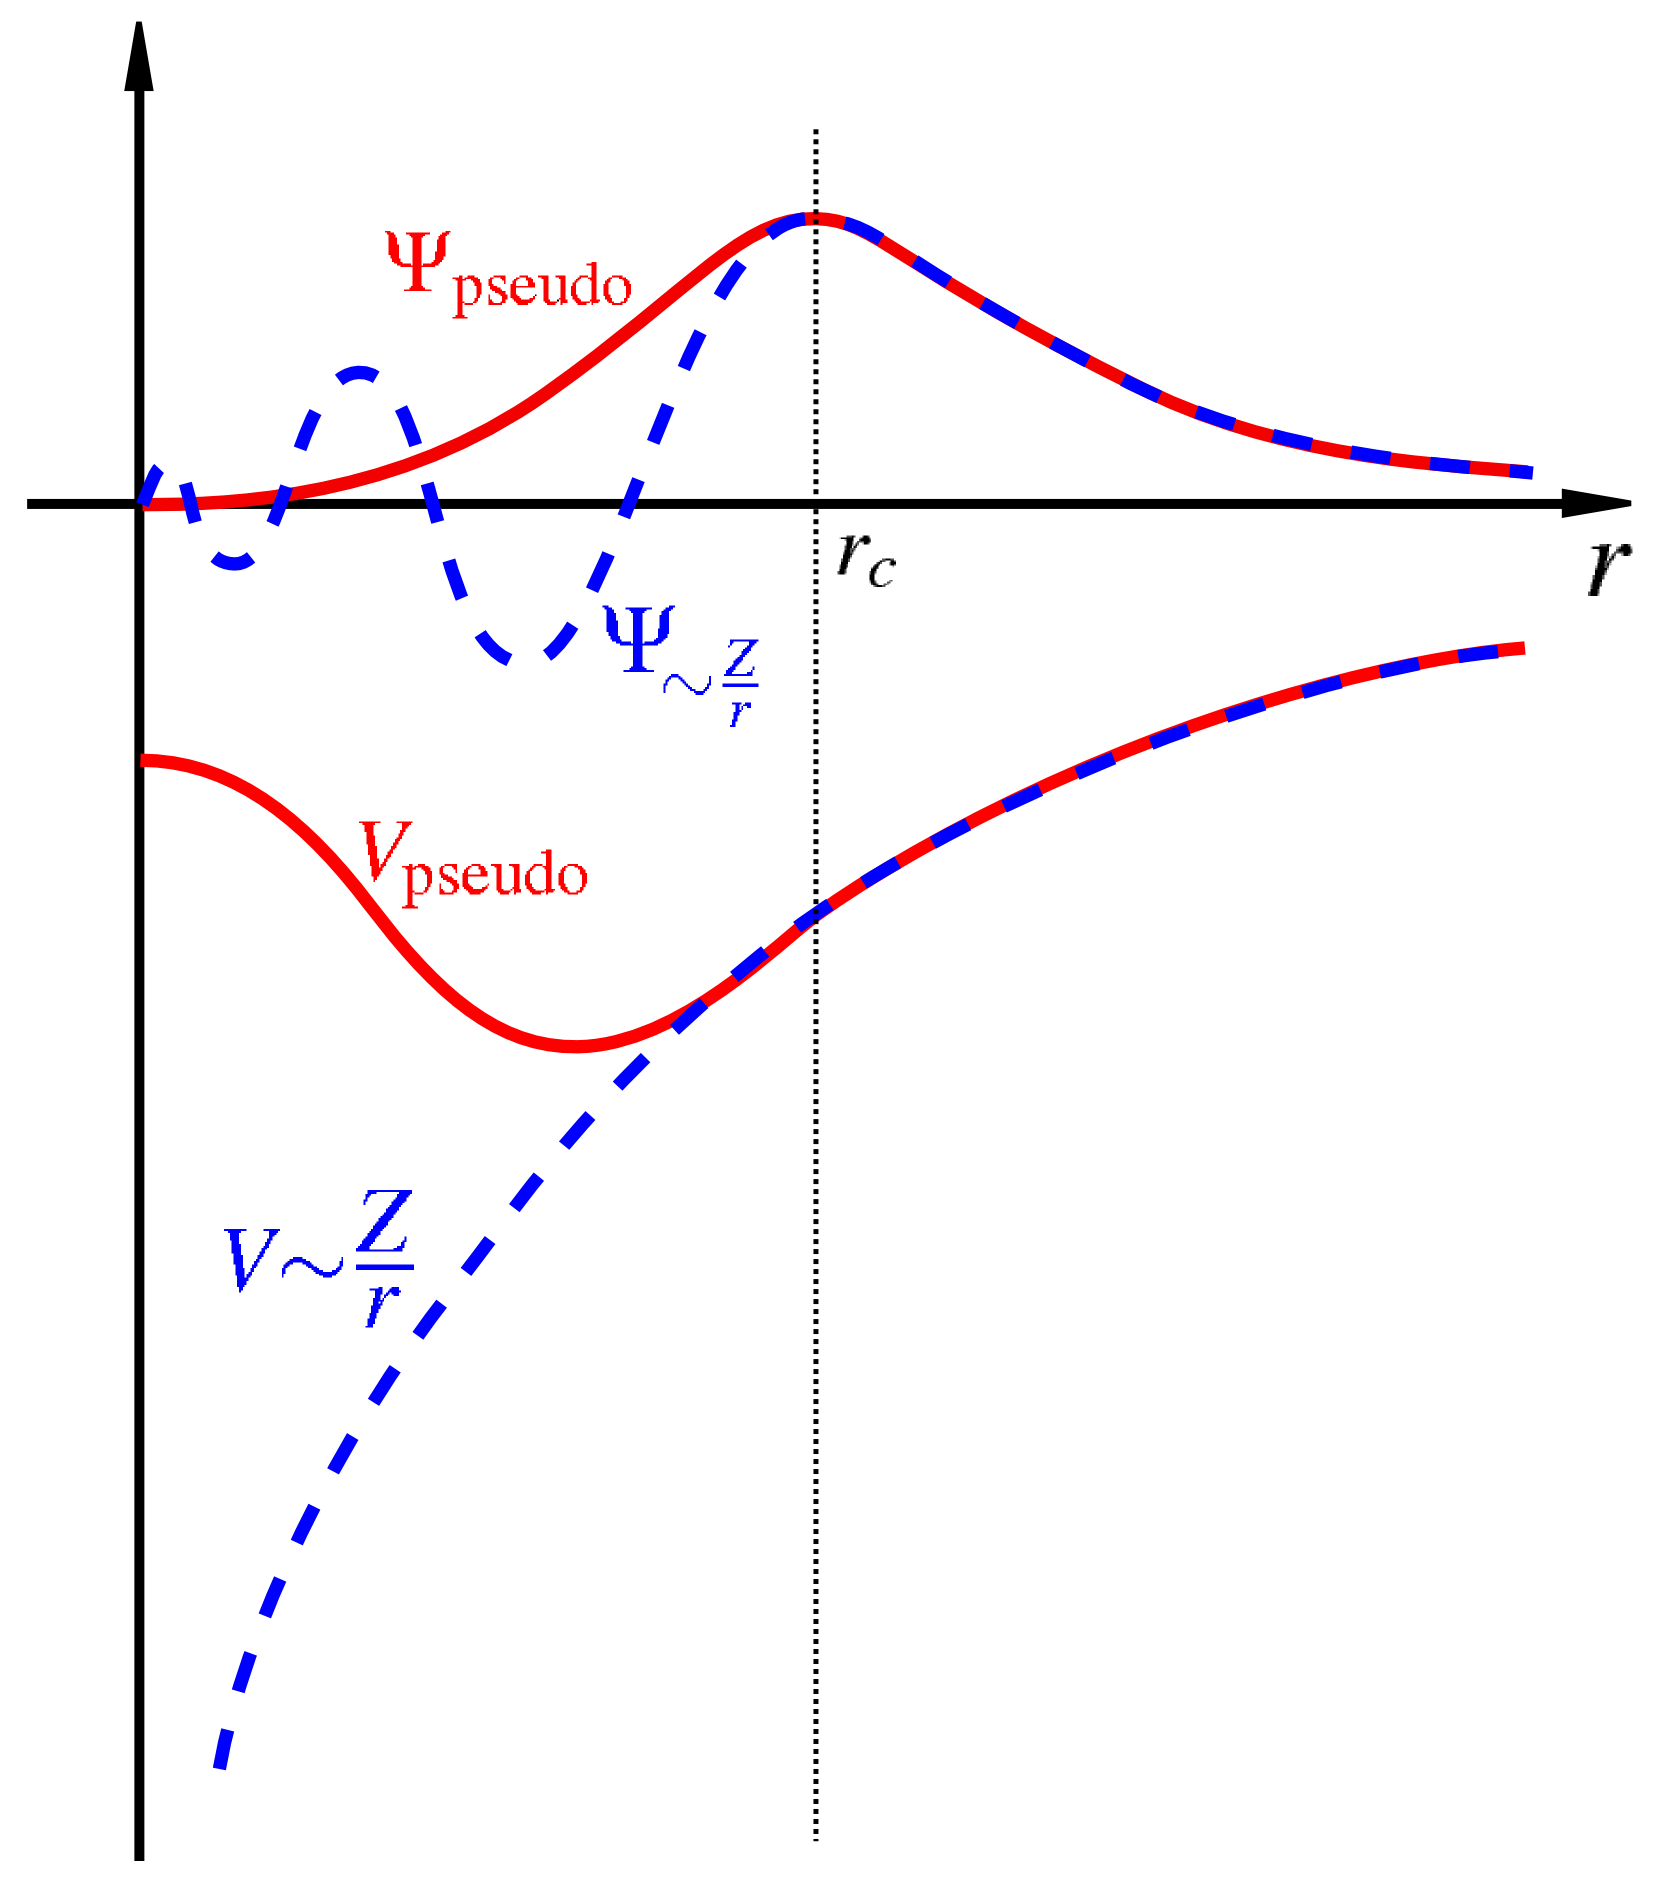
\includegraphics[width=0.5\textwidth]{Sketch_Pseudopotentials.png}
	\caption{Sketch of the pseudopotential compared to the real potential and the wavefunctions they generate.}
	\label{fig:sketch_pseudo}
\end{figure}
Beyond a given cutoff radius $r_c$, pseudopotentials are constrained to be exactly equal to the true potential. Below this radius, the pseudopotential does not diverge and assumes a finite value at $r=0$, as can be seen in Fig. \ref{fig:sketch_pseudo} This generates a pseudo-wave function which is smooth and does not oscillate below the cutoff radius. With this method, the Kohn-Sham eigenvalues remain unchanged, and the computationally demanding task of representing the oscillating wave function is eliminated. The fact that fewer electrons have to be taken into account also helps to speed up the calculations.
%

\subsubsection{Basis set}
For real systems, the wave function of the crystal is an immensely complicated object whose analytical expression is out of reach. For computational purposes, one needs to represent it in a complete basis of the Hilbert space. Depending on the characteristics of the system, the choice of the basis functions is different.

In this thesis we study infinite, periodic crystals. A suitable basis for this case is the plane waves. It originates naturally from the Bloch theorem, which states that the wave function of an electron can be written as a product of a plane wave times a periodic function :
\be
 	\phi_{j,\kk} (\rr) = u_j (\rr) e^{i\kk\cdot\rr}
\ee
The $u_j$ functions have the same periodicity as the lattice. The plane wave has a wavevector $\kk$. For infinite periodic crystals, this is a continuous variable belonging in the first \acrfull{BZ}. The quantity $\hbar \kk$ is called the quasi-momentum of the electron, or \textit{crystal momentum}. For brevity, we will sometimes call it momentum of the electron.
We decompose the periodic functions $u_j$ in plane waves as such :
\be
 	u_j (\rr) = \sum_{\GG} c_{j,\GG} e^{i\GG \cdot \rr}
\ee
where $c_{j,\GG}$ are the coefficients of the plane waves basis, and the $\GG$ are the reciprocal lattice vectors. The plane waves expansion of the band $j$ follows :
\be
	\phi_{j,\kk} (\rr) = \sum_{\GG} c_{j,\kk+\GG} e^{i (\kk+\GG)\cdot \rr}
\ee
In principle all complete bases of the Hilbert space yield equal representation of the wave function. As it is impossible to numerically sample a Hilbert space with infinite dimension, one has to truncate the representation. Thus, one has to make sure enough basis functions are included in the expansion to have an accurate wave function. In our case, we choose an energy cutoff $E_{cut}$ such that :
\be
	\frac{1}{2} \left| \kk+\GG \right|^2 \leq E_{cut}
\ee
One has to verify that the cutoff is high enough so that the results are accurate, but setting it too high would mean including more plane waves which would slow down the calculations. Since the plane waves are orthonormal, adding extra ones to the basis by increasing $E_{cut}$ does not add redundant physical information. \cite{martin2020electronic} All the potentials entering the Kohn-Sham equations can be expressed in the plane waves basis, as well as the equations themselves.



%%%%%%%%%%%%%%%%%%%%%%%%%%%%%%%%%%%%%%%%%%%%%%%%%%%%%%%%%%%%%%%%%%%%%%%%%%%%%%%%%%%%%%%%%%%%%%%%
%%%%%%%%%%%%%%%%%%%%%%%%%%%%%%%%%%%%%%%%%%%%%%%%%%%%%%%%%%%%%%%%%%%%%%%%%%%%%%%%%%%%%%%%%%%%%%%%
%

\section{Many-Body Perturbation Theory}
As mentioned above, \acrshort{DFT} is not well suited to simulate optics experiments of semiconductors or insulators. Optical excitations are neutral excitations, in the sense that the excited electron does not leave the system and can therefore interact with the hole it left behind in the valence band. This interaction between a hole in a valence band and an excited electron in the conduction bands is not accurately accounted for in \acrshort{DFT}, as it is designed to calculate the total energy and the electronic density of the \textit{groundstate}. For this reason, we resort to a more refined theoretical framework to treat the electronic correlations and study the excited states.

In this section I will present the basics of \acrfull{MBPT}. In this theory, the many-body interactions are treated as a perturbation to the system of non-interacting electrons. I will detail the effects on the electronic structure and also the inclusion of the electron-hole interaction, to deal with optical excitations. \\
Including the many-body interaction in an Hamiltonian formulation would lead to computing immensely complicated wavefunctions for the system of N electrons, and this is not tractable. Instead, if we are more interested in observables such as optical spectra, we can reformulate the problem in terms of Green's functions. It is a mathematical object which is the solution of the equation of motion for the N interacting electrons, when the source term is a Dirac distribution. The link between the two formulation writes :
\begin{align}
\begin{split}
	&\left[ i \partial_t - \hat{H}_e \right] \mathcal{G}(\rr,t;\rr',t') = \delta(\rr-\rr')\delta(t-t') \\
	&\mathcal{G}(\rr,\rr',\omega) = \left[\omega - \hat{H}_e\right]^{-1}
\end{split}	
\end{align}
The first line is the time-dependent Schrödinger equation for N interacting electrons. The second line gives the N-body Green's function in terms of the Hamiltonian, where we took the Fourier transform $t-t' \to \omega$. The one-body and two-body Green's functions are the first two matrix elements of $\mathcal{G}$. We will see in this section how to obtain many useful quantities from them, such as the electronic density, the total energy, the charged and neutral excitation energies and much more. 
The derivations in this section are adapted from textbooks,\cite{martin2016interacting,stefanucci2013nonequilibrium} review articles \cite{strinati1988application,aryasetiawan1998gw,giustino2017review} and lecture notes.\cite{JulienToulouseNotes}

\subsection{Hedin's equations}
We consider a system of N interacting electrons. We will consider the effect of nuclei motion in a later section.
We start from the Hamiltonian for interacting electrons in second quantization:
\begin{align}
\begin{split}
 	\hat{H} &= \int dx_1 \ \hpsidag(x_1) h(\rr_1) \hpsi(x_1) + \frac{1}{2} \iint dx_1 \  dx_2 \ \hpsidag(x_1) \hpsidag(x_2) v(\rr_1,\rr_2) \hpsi(x_2)\hpsi(x_1) \\
		&= \hat{H}_0 + \hat{H}_{int}.
\end{split}
\end{align}
where $\hat{\psi}(x)$ is a field operator in Schrödinger representation, $h$ is the single-particle Hamiltonian for non-interacting particles evolving in an external potential $V_{ext}$ and $v(\rr_1,\rr_2) = e^2 (\left| \rr_1 - \rr_2 \right|)^{-1}$ is the Coulomb interaction. In the above equation, $x$ is the combined space and spin variables $x = (\rr, \sigma)$.
%

For the following derivation, we introduce an external potential $\Phi(x,x';t)$ which is local in time but nonlocal in space. We write it in the form of an interaction Hamiltonian :
\begin{equation}
	\hat{H}'(t) = \int dx dx' \hpsidag(x) \Phi(x,x';t) \hpsi(x') 
\end{equation}
In our case, this external perturbation will be set to 0 at the end of the calculation. It is a formal tool to derive the useful equations for the time-evolution of Green's functions. With this Hamiltonian, it is especially relevant to introduce the \textit{interaction picture}, in which both the operators and the wavefunctions have a time dependence.\cite{martin2016interacting} For the field operators we have :
\begin{equation}
	\hpsi(1) \equiv \hpsi(x_1, t_1) = e^{i\hat{H} t_1} \hpsi(x_1) e^{-i\hat{H} t_1}
\end{equation}
and for the interaction Hamiltonian :
\begin{equation}
	\hat{H}_I'(t) = e^{i\hat{H} t} \hat{H}'(t) e^{-i\hat{H} t} = \int dx dx' \hpsidag(x,t^+) \Phi(x,x';t) \hpsi(x',t)
\end{equation}
where we use the notation $t^+$ for $t+\delta (\delta \to 0^+)$. We define a time-evolution operator in terms of this interaction Hamiltonian :
\begin{equation}
	\hat{S} = \exp\biggl\{ -i \int_{-\infty}^{+\infty} dt \hat{H}_I'(t) \biggr\} \label{eq:def_time_ev_op}
\end{equation}
We now write the definitions of single- and two-particle Green's functions that include the dependence in $\Phi$ :
\begin{equation}
	G(1,2) = -i \frac{\bra{N}\hat{T}\left[\hat{S}\hpsi(1)\hpsidag(2)\right]\ket{N}}{\bra{N}T[\hat{S}]\ket{N}} \label{eq:GF}
\end{equation}
and
\begin{equation}
	G_2(1,2:1',2') = (-i)^2  \frac{\bra{N}\hat{T}\left[\hat{S}\hpsi(1)\hpsi(2)\hpsidag(2')\hpsidag(1')\right]\ket{N}}{\bra{N}T[\hat{S}]\ket{N}}\label{eq:2GF}
\end{equation}
where $\ket{N}$ is the exact ground state of the N-electron system and T is a time-ordering operator. It ensures that the time variable increases from right to left. It gives $\hat{T}\left[ \hpsi(\rr_1 t_1) \hpsidag(\rr_2 t_2) \right] = \theta(t_1 - t_2) \hpsi(\rr_1 t_1) \hpsidag(\rr_2 t_2) - \theta(t_2-t_1)\hpsidag(\rr_2 t_2)\hpsi(\rr_1 t_1)$, where $\theta$ is the Heaviside function.\cite{fetter2012quantum} The physical meaning of the one-body Green's function is the probability amplitude that an electron added in the system at time $t_2$ and position $\rr_2$ propagates to position $\rr_1$ and time $t_1$. In the time-ordered formalism that we are using, it is also the probability amplitude that a hole created at time $t_1$ and position $x_1$ propagates to $(x_2,t_2)$, depending on how the two time variables are ordered. \textcolor{red}{maybe add a figure to illustrate}
The two-particle Green's function $G_2$ describes the propagation of two correlated particles. Depending on the time ordering, it can describe a propagation electron-electron pair, a hole-hole pair or an electron-hole pair. It will become useful in a following section. \\
%

We will now sketch a derivation for the equations of motion for the single-particle Green's function. To do this, we will make explicit the time dependence of each term in Eq. \eqref{eq:GF}.
We start with the time evolution of the quantity $\hat{T}[\hat{S}]$ appearing in the denominator of Eq. \eqref{eq:GF}.
For this we define the time evolution operator from Eq. \eqref{eq:def_time_ev_op} in the interaction picture, from time $t_a$ to $t_b$ :
\begin{equation}
	\hat{S}(t_a,t_b) = \exp	\biggl\{ -i \int_{t_a}^{t_b} dt \hat{H}_I'(t) \biggr\}
\end{equation}
Now the time derivatives of $\hat{T}[\hat{S}]$ are:
\begin{align}
\begin{split}
	\frac{\partial}{\partial t_a} T[\hat{S}(t_a,t_b)] &= -i \hat{H}'_I(t_a)T[\hat{S}(t_a,t_b)] \\
	\frac{\partial}{\partial t_b} T[\hat{S}(t_a,t_b)] &= i T[\hat{S}(t_a,t_b)]\hat{H}'_I(t_b)
\end{split}
\end{align}
For the field operators, the derivation of the equations of motions can be found in Appendix \ref{app:EOM}. They read :
\begin{align}
\begin{split}
	\frac{\partial}{\partial t_1} \hpsi(1) &= -i \left[ h(1) + \int d3 v(1,3) \hpsidag(3)\hpsi(3) \right] \hpsi(1) \\
	\frac{\partial}{\partial t_2} \hpsidag(2) &= i \left[ \hpsidag(2)h(2) + \hpsidag(2) \int d3 v(2,3) \hpsidag(3)\hpsi(3) \right]
\end{split}	
\end{align}
where we introduced $v(1,2) = v(\rr_1,\rr_1)\delta(t_1-t_2)$ and $h(1)=h(\rr_1)$. Knowing that the derivative of the Heaviside function is a Dirac delta, we can write the equations of motion for the single-particle Green's functions :
\begin{align}
\begin{split}
	&\left[ i\frac{\partial}{\partial t_1} - h(1) \right] G_1(1,2) - \int d3 \Phi(1,3)G_1(3,2) + i \int d3 v(1,3) G_2(1,3^+;2,3^{++}) = \delta(1,2) \\
	&\left[ -i\frac{\partial}{\partial t_2} - h(2) \right] G_1(1,2) - \int d3 G_1(1,3)\Phi(3,2) + i \int d3 v(2,3) G_2(1,3^{--};2,3^-) = \delta(1,2)
\end{split}
\end{align}
with the notations : 
\begin{equation}
	\Phi(1,2) = \Phi(x_1,x_2;t_1) \delta(t_1-t_2).
\end{equation}
and 
\begin{equation}
	1^+ = (r_1,t_1^+) \ \text{where} \ t_1^+ = \lim_{\eta \to 0} t_1 + \eta, \qquad \eta > 0
\end{equation}
and equivalently for $1^{++}$ and $1^-$.
Here we notice that the equations for the single-particle Green's function depend on the two-particle Green's function. The latter could be expressed in terms of the three-body Green's function, and so on. Instead of using a hierarchy of higher-order Green's function, we will eliminate the two-particle Green's function from the equation and write a set of coupled integro-differential equations containing the self-energy and other useful quantities.
%

We use the functional derivative identity, derived for example in Ref. \cite{strinati1988application} :
\begin{equation}
	G_2(1,3;2,3^+) = G(1,2)G(3,3^+) - \frac{\delta G(1,2)}{\delta \Phi(3)} \label{eq:2GF_dPhi}
\end{equation}
where we consider the external potential to be local in space $\Phi(x_1,x_2;t_1) \\ = \Phi(x_1,t_1)\delta(x_1,x_2)$. This restriction is enough to generate the equations of motion for the single-particle Green's function. For the two-particle ones instead, one needs to consider the more general form of the external potential, non-local in space.
The equations of motion become :
\begin{multline}
	\left[ i \frac{\partial}{\partial t_1} - h(1) - \Phi(1) + i \int d3 v(1,3)G(3,3^+) \right] G(1,2) \\ 
	- i \int d3 v(1^+,3) \frac{\delta G(1,2)}{\delta \Phi(3)} = \delta(1,2)
\end{multline}
and
\begin{multline}
	\left[ i \frac{\partial}{\partial t_2} - h(2) - \Phi(2) + i \int d3 v(2,3)G(3^-,3) \right] G(1,2) \\
	- i \int d3 v(2^-,3) \frac{\delta G(1,2)}{\delta \Phi(3)} = \delta(1,2)
\end{multline}
We cannot take the limit $\Phi \to 0$ yet because it would require the knowledge of the functional dependence of $G$ on $\Phi$. However Hedin proposed a way to rewrite the equations of motion (or at least one of them and the other would undergo the same process) by introducing new physical quantities, coupled in nonlinear self-consistent equations.\cite{hedin1965new} 
%

The first of these quantities is the \textbf{total classical potential} $V$ : 
\begin{equation}
	\vtot (1) \equiv \int d2 v(12) \langle \hat{n}(2) \rangle + \Phi(1) \label{eq:vtot}
\end{equation}
where $\hat{n}$ is the density operator. It is the total potential felt by the electrons. It is local as is it the sum of the external perturbation and the Hartree potential. The equation of motion for the Green's function is then :
\begin{equation}
	\left[ i \frac{\partial}{\partial t_1} + \frac{1}{2}\nabla^2(1) - \vtot (1) -i\int d3 v(1^+,3) \frac{\delta}{\delta \Phi(3)} \right] G(1,2) = \delta(1,2) \label{eq:GF_EOM}
\end{equation}
To get rid of the functional derivative with respect to the external perturbation, we make use of the definition of the inverse Green's function and of the functional differentiation of a product:
\begin{equation}
	\frac{\delta G(1,2)}{\delta \Phi(3)} = - \int d45 G(1,4) \frac{\delta G^{-1}(4,5)}{\delta \Phi(3)} G(5,2)
\end{equation}
where the inverse single-particle Green's function is defined as :
\begin{equation}
	\int d3 G^{-1}(1,3) G(3,2) = \int d3 G(1,3)G^{-1}(3,2) = \delta(1,2) \label{eq:inv_GF}
\end{equation}
We now use the chain rule for functional differentiation :
\begin{equation}
	\frac{\delta G^{-1}(4,5)}{\delta \Phi(3)} = \int d6 \frac{\delta G^{-1}(4,5)}{\delta \vtot(6)} \frac{\delta \vtot(6)}{\delta \Phi(3)}
\end{equation}
We introduce the \textbf{scalar vertex function}, a three-point quantity defined as :
\begin{equation}
	\Gamma(1,2;3) \equiv -\frac{\delta G^{-1}(1,2)}{\delta \vtot(3)} \label{eq:vertex}
\end{equation}
We introduce the \textbf{inverse dielectric matrix} $\inveps$ :
\begin{equation}
	\inveps(1,2) = \frac{\delta \vtot(1)}{\delta \Phi(2)}.
\end{equation} 
It is the many-body formulation of the classical (inverse) dielectric matrix. 
We introduce the \textbf{dynamically screened interaction} $W$ or screened Coulomb interaction, defined as :
\begin{equation}
	W(1,2) \equiv \int d3 \inveps(1,3) v(3,2) \equiv \int d3 v(1,3) \inveps(2,3)
\end{equation}
\textcolor{red}{add a Feynman diagram to illustrate}
Note that the screened interaction is symmetric under the exchange of indices $W(1,2) = W(2,1)$.
Finally, we introduce the \textbf{electron self-energy}, defined as :
\begin{equation}
	\Sigma(1,2) = i \int d34 G(1,3) \Gamma(3,2;4) W(4,1^+)
\end{equation}
%

With these quantities, we can rewrite the equation of motion for the single-particle Green's function :
\begin{equation}
	\left[ i \frac{\partial}{\partial t_1} + \frac{1}{2}\nabla^2(1) - \vtot (1)\right] G(1,2) - \int d3 \Sigma(1,3) G(3,2) = \delta(1,2) \label{eq:GF_EOM_SE}
\end{equation}
We can see here that the self-energy $\Sigma$ has the meaning of a non-local and energy-dependent effective single-particle potential.
%

Using Eqs. \eqref{eq:vertex} and \eqref{eq:GF_EOM_SE}, we can express the vertex function in terms of the above quantities. 
\begin{equation}
	\Gamma(1,2;3) = \delta(1,2) \delta(1,3) + \int d4567 \frac{\delta \Sigma(1,2)}{\delta G(4,5)} G(4,6) G(7,5) \Gamma(6,7;3). \label{eq:vertex_hedin}
\end{equation}
More details about these quantities and their derivations can be found for example in Strinati's review. \cite{strinati1988application}
The previous quantities form a set of coupled integro-differential equations. In order to close the loop and build a self-consistent set, we need to write the relations between $W$ and the other quantities. By combining $\vtot$, $\inveps$ and $W$, we get :
\begin{equation}
	W(1,2) = v(1,2) + \int d34 v(1,3) \frac{\delta \langle \hat{n}(3)\rangle}{\delta \vtot (4)} W(4,2)
\end{equation}
We define the \textbf{irreducible polarizability} to be :
\begin{equation}
	\tilde{\chi}(1,2) \equiv \frac{\delta \langle \hat{n}(1)\rangle}{\delta \vtot (2)}. \label{eq:P_dn/dV}
\end{equation}
It is the response of the density under the action of the total classical potential. This term is often called $P$ in the $GW$ literature. The reducible polarizability is instead the derivative of the density with respect to the perturbation $\Phi$ :
\begin{align}
	&\chi(1,2) \equiv \frac{\delta \langle \hat{n}(1)\rangle}{\delta \Phi (2)}\\
	 &= \int d3 \frac{\delta n(1)}{\delta \vtot(3)} \frac{\delta \vtot(3)}{\delta \Phi (2)} = \int d3 \tilde{\chi}(1,3)\inveps(3,2) = \tilde{\chi}(1,2) + \int d34 \tilde{\chi}(1,3) v(3,4) \chi(4,2) \label{eq:chi_dn/dPhi}
\end{align}

With the following relation 
\begin{equation}
	n(1) = \langle \hat{n}(1)\rangle = -iG(1,1+),
\end{equation}
and using properties of the inverse Green's function and the chain rule, one can write :
\begin{align}
\begin{split}
	\tilde{\chi}(1,2) &= -i \frac{\delta G(1,1+)}{\delta \vtot(2)} = i \int d34 G(1,3)\frac{\delta G^{-1}(3,4)}{\delta \vtot(2)}G(4,1^+)\\
	&= -i \int d34 G(1,3) G(4,1^+) \Gamma(3,4;2) \label{eq:tilde_chi}
\end{split}
\end{align}
Then we can write the screened interaction in term of $\tilde{\chi}$ :
\begin{equation}
	W(1,2) = v(1,2) + \int d34v(1,3)\tilde{\chi}(3,4) W(4,2)
\end{equation}
as well as the dielectric matrix :
\begin{equation}
	\epsilon(1,2) = \delta(1,2) - \int d3 v(1,3) \tilde{\chi}(3,2)
\end{equation}
Note that we can also express the \textit{inverse} dielectric matrix in terms of the reducible polarizability from Eq. \eqref{eq:chi_dn/dPhi} :
\begin{equation}
	\epsilon^{-1}(1,2) = \delta(1,2) + \int d3 v(1,3) \chi(3,2)
\end{equation}
where both quantities satisfy :
\begin{equation}
	\int d3 \epsilon^{-1}(1,3)\epsilon(3,2) = \int d3 \epsilon(1,3)\epsilon^{-1}(3,2) = \delta(1,2).
\end{equation}
We now have a set of coupled self-consistent equations, where the limit $\Phi \to 0$ can be taken. 
%

\subsection{Dyson equation}

In order to be able to compute the Green's function and the related useful quantities, we need to reformulate the problem using the non-interacting Green's function $G_0$. We start by separating the part which comes only from the one-particle operators in the equation of motion Eq. \eqref{eq:GF_EOM_SE} :
\begin{equation}
	\left[ i\frac{\partial}{\partial t_1} - h(1) \right] G_0(1,2) = \delta(1,2)
\end{equation}
This is the definition of the non-interacting Green's function $G_0$. Using its inverse $G_0^{-1}$, which obeys the same relation as the full single-particle Green's function in Eq. \eqref{eq:inv_GF}, we can rewrite the interacting Green's function as :
\begin{equation}
	G(1,2) = \int d34 G_0(1,4)G^{-1}_0(4,3)G(3,2)
\end{equation}
Inserting the above equation in Eq. \eqref{eq:GF_EOM_SE}, we get :
\begin{equation}
	\int d3 \left[ G_0^{-1}(1,3) - \Sigma(1,3) \right] G(3,2) = \delta(1,2).
\end{equation}
After multiplying the from the left by $\int d1 G_0(4,1)$ we obtain :
\begin{equation}
	G(1,2) = G_0(1,2) + \int d34 G_0(1,3) \Sigma(3,4) G(4,2) \label{eq:Dyson}
\end{equation}
or equivalently,
\begin{equation}
	G^{-1}(1,2) = G_0^{-1}(1,2) - \Sigma(1,2)
\end{equation}
Equation \eqref{eq:Dyson} is called the \textit{Dyson equation} for the single-particle Green's function. Knowing $G_0$, which is numerically simple to compute, and approximating the self-energy $\Sigma$, which we will discuss later, allows one to compute the Green's function $G$. At this point it is useful to rewrite the self-energy as a sum of two terms $\gS = v_H + \gS_{xc}$, which are the Hartree potential and the exchange-correlation self-energy. Formally, it writes :
\begin{equation}
	\gS(1,2) = v_H(1,2) - i\int d34 v(1,4)G(1,3) \left[ \frac{\delta G^{-1}(3,2)}{\delta \Phi(4^+)} \right] 
\end{equation}
\textcolor{red}{add a Feynman diagram to illustrate}
%
\subsection{Random Phase Approximation} 
The \acrfull{RPA} consists in neglecting the vertex corrections in the formula of the reducible polarizability Eq. \eqref{eq:tilde_chi}. The vertex functions is reduced to 
\begin{equation}
	\Gamma(1,2;3) \approx \delta(1,2)\delta(1,3).
\end{equation}
Then the irreducible polarizability writes :
\begin{equation}
	\tilde{\chi}(1,2) \approx \tilde{\chi}_0(1,2) \equiv -i G(1,2^+)G(2,1^+) \label{eq:tilde_chi_0}
\end{equation}
% I use \tilde{\chi} and not \chi to be consistent with the definition in Hedin's equations.
Working out the above expression, one can see that it is made of non-interacting electron-hole pairs. The full polarizability follows from Eq. \eqref{eq:chi_dn/dPhi} :
\begin{equation}
	\chi(1,2) = \tilde{\chi}_0(1,2) + \int d34 \tilde{\chi}_0(1,3) v(3,4) \chi(4,2) = \int d3 \tilde{\chi}_0(1,3) \left[ 1 - v \tilde{\chi}_0\right]^{-1}(3,2)
\end{equation}
When we calculate $\tilde{\chi}_0$ from the single-particle Green's function as in Eq. \eqref{eq:tilde_chi_0}, the derivative with respect to the perturbation is neglected. In this regard, $\tilde{\chi}_0$ is not an \acrshort{RPA} response function. We call it the independent particle response function while $\tilde{\chi}$ is called the RPA response function, for historical reasons.
However, $\tilde{\chi}_0$ will be useful when dealing with optical properties. Indeed, from the inverted form, one can construct the inverse dielectric function, written in a compact form as $\inveps = 1+v \chi^{RPA}$.

%
\subsection{The $GW$ approximation}
With the Dyson equation for the Green's function, we can now complete the set of self-consistent, coupled equations that are called the \textit{Hedin's equations} \cite{hedin1965new}:
\begin{empheq}[box=\widefbox]{align*}
	&\Sigma(1,2) = i \int d34 G(1,3) \Gamma(3,2;4) W(4,1^+) \\
	&G(1,2) = G_0(1,2) + \int d34 G_0(1,3) \Sigma(3,4) G(4,2) \\
	&\Gamma(1,2;3) = \delta(1,2) \delta(1,3) + \int d4567 \frac{\delta \Sigma(1,2)}{\delta G(4,5)} G(4,6) G(7,5) \Gamma(6,7;3) \\ 
	&\tilde{\chi}(1,2) = -i \int d34 G(1,3) G(4,1^+) \Gamma(3,4;2) \\
	&W(1,2) = v(1,2) + \int d34v(1,3)\tilde{\chi}(3,4) W(4,2)
\end{empheq}
$\Gamma$ and $W$ also satisfy Dyson equations, just as $G$. This is an exact set of coupled equations, that is solved self-consistently. In practice, it is untractable to solve. One has to chose a starting approximation for the self-energy, which contains the summation to all orders in the interaction expansion of $G$. One way to approximate the self-energy is to consider $\frac{\delta \Sigma(12)}{\delta G(4,5)} = 0$ so that $\Gamma = \delta(1,2)\delta(1,3)$ and we obtain :
\begin{equation} 
\gS_{xc}(1,2) = iG(1,2)W(1,2). \label{eq:GW}
\end{equation}
This is the so-called $GW$ approximation, which gives good results for weakly-correlated materials. \cite{aryasetiawan1998gw} It is the first-order in the expansion of the self-energy in terms of the interaction $W$. All higher order terms that are involved in electronic correlations are neglected. Part of those can be included by recomputing $G$ self-consistently with the Hedin's equations. However in practice, it is not guaranteed that it leads to better results. Most of the times, the $GW$ method is a one-shot calculation starting from the DFT Kohn-Sham eigenvalues and wave functions, as we will see in a later subsection. 

Eq. \eqref{eq:GW} resembles the Hartree-Fock approximation, where the exchange part of the self-energy is written as $\gS_x^{HF}(1,2) = i G(1,2^+)v(1,2)$.
The difference in this case is that we used the dynamically screened interaction instead of the bare Coulomb one. 

%
\subsection{Quasiparticle equations}
Once the limit $\Phi \to 0$ is taken, there is no time-dependent potential acting on the system of N electrons. Hence, the system is invariant under time translation and the Green's function depends only on the time difference $\tau = t_1 - t_2$. One can do the Fourier transform from time $\tau$ to frequency $\omega$, and we can write the Green's function in the so-called Lehmann representation :
\begin{equation}
	G(x_1,x_2;\omega) = \sum_a \frac{f_a(x_1)f_a^*(x_2)}{\omega-\epsilon_a + i\eta} + \sum_i \frac{f_i(x_1)f_i^*(x_2)}{\omega-\epsilon_i + i\eta}
\end{equation}
where $a,i$ denote electron states, $f_a(x) = \bra{N}\hpsi(x)\ket{N+1,a}$ and \\ $f_i(x) = \bra{N-1,i} \hpsi(x) \ket{N}$ are the Lehmann amplitudes (also called Dyson orbitals). They are defined with the $N$-electron ground state $\ket{N}$ whose total energy is $E_N$, the electron state number $a$ of the $(N+1)$-electron system $\ket{N+1,a}$ with total energy $E_{N+1,a}$ and the electron-state number $i$ of the $(N-1)$-electron system $\ket{N-1,i}$ with total energy $E_{N-1,i}$.
The Lehmann representation of the Green's function also contains the quasiparticle energies, which are defined as $\epsilon_a = E_{N+1,a} - E_N = -A_a$ and $\epsilon_i = E_N - E_{N-1,i} = -I_i$. $A_a$ and $I_i$ are the electron affinities and ionization energies. This highlights the link between the poles of the Green's function from many-body perturbation theory and the \acrfull{PES} and \acrfull{IPES}, and is illustrated in Fig. \ref{fig:sketch_PES}. In \acrshort{PES}, the ionization energy writes $I_i = -\epsilon_i = \hbar \omega - E_{kin} - \Phi$ for $\epsilon_i < E_F$ where $\Phi$ is the extraction energy to send an electron above the vacuum energy $E_{vac}$ with a kinetic energy $E_{kin}$, thanks to an irradiation of energy $\hbar \omega$. In \acrshort{IPES}, the electronic affinity writes $-A_a = \epsilon_a = E_{kin} - \hbar \omega + \Phi$, for $\epsilon_a \geq E_F$.
\begin{figure}[tbp]
	%\vspace{0.5cm}
	\setcapindent{2em}
	\centering
	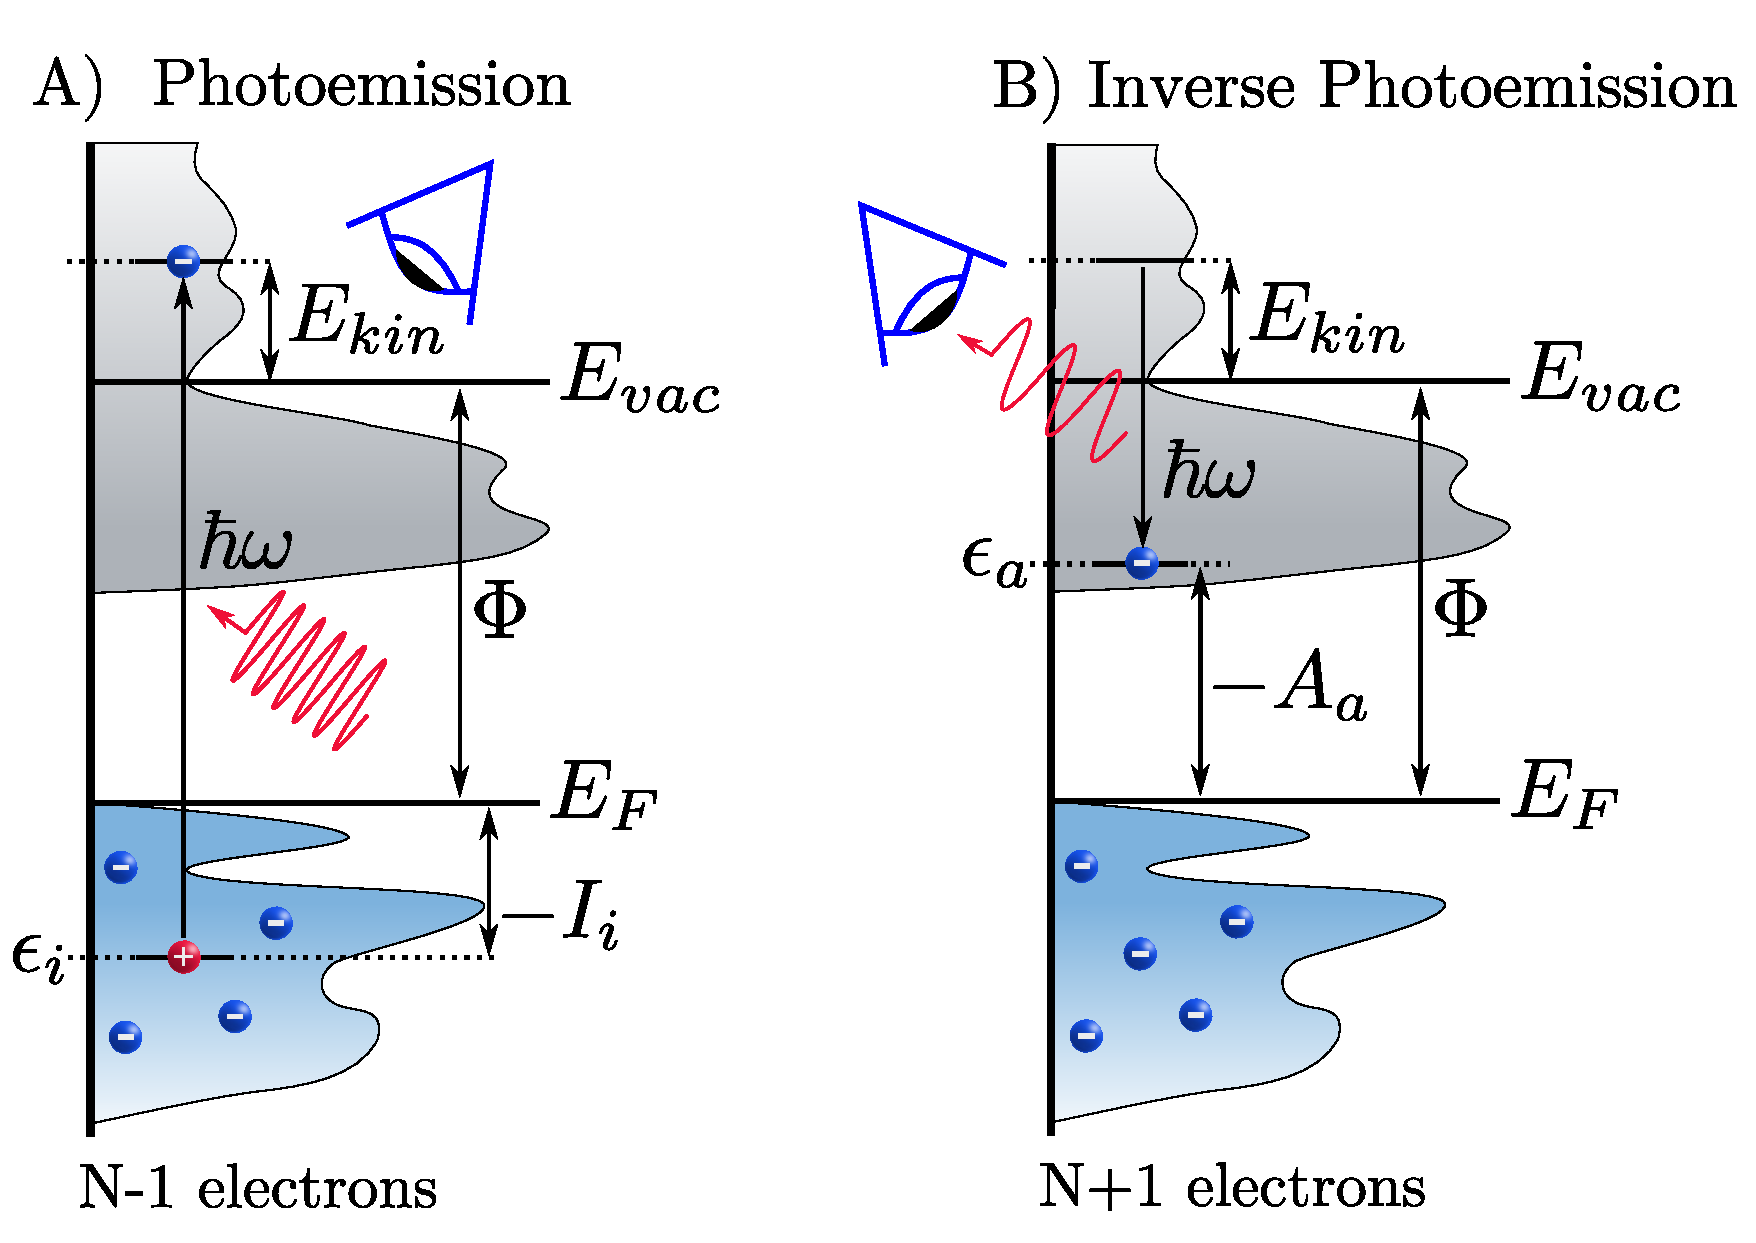
\includegraphics[width=0.8\textwidth]{PES_IPES.pdf}
	\caption{Sketches of A) the photoemission spectroscopy , where the kinetic energy of the extracted electron is measured, B) Inverse photoemission spectroscopy, where the emitted light coming from the de-excitation of the added electron is measured. $E_F$ is the Fermi level, $E_{vac}$ is the vacuum level, $E_{kin}$ is the kinetic energy of the added or removed electron, $\Phi$ is the extraction energy. }
	\label{fig:sketch_PES}
\end{figure}

With this form of the Green's function we can reformulate the Dyson equation Eq. \eqref{eq:Dyson}. Just as the Green's function, the self-energy depends only on the time difference $\tau = t_1 - t_2$. We can then take the Fourier transform of Eq. \eqref{eq:GF_EOM_SE} :
\begin{equation}
	\left[ \omega - h(\rr_1) \right] G(x_1,x_2;\omega) - \int dx_3 \Sigma(x_1,x_2;\omega) G(x_3,x_2;\omega) = \delta(x_1,x_2)
\end{equation}
Inserting the Lehmann representation of $G(x_1,x_2;\omega)$, one can select the term corresponding to a given pole $\epsilon_n$ by multiplying the equation by $\omega - \epsilon_n$ and taking the limit $\omega \to \epsilon_n$, giving :
\begin{equation}
	\left[ \epsilon_n - h(\rr_1) \right] f_n(x_1)f^*_n(x_2) - \int dx_3 \Sigma(x_1,x_3;\epsilon_n) f_n(x_3) = \epsilon_n f_n(x_1)
\end{equation}
and we obtain an eigenvalue equation :
\begin{equation}
	h(\rr_1)f_n(x_1) + \int dx_3 \Sigma(x_1,x_3;\epsilon_n)f_n(x_3) = \epsilon_n f_n(x_1)
\end{equation}
These are the \textit{quasiparticle equations}. They give the quasiparticle energies and the Lehmann amplitudes, or also called the Dyson orbitals. The quasiparticle energies are in general complex, and the Lehmann amplitudes, which act as the quasiparticles wavefunctions, are not orthogonal because $\Sigma$ is energy-dependent and non Hermitian. The physical meaning of the poles of $G$ is therefore the exact excitation energies of the $N\pm1$ electrons. In an infinite, periodic system, the poles form a branch cut, and we can interpret the excitation spectrum in terms of quasiparticles with energies $\Re\epsilon_n$ and life-times $1/\Im\epsilon_n$
Here it is made apparent that $\Sigma$ is a non-local, energy-dependent single-particle effective potential. One thing to notice is also the fact that the quasiparticle energy is made out of the bare, independent single particle, and another term coming from the interaction with surrounding particle. The quasiparticle is the bare particle "dressed" with the interaction. This is a formulation in the Green's functions formalism of the quasiparticle concept, which was first introduced by Landau in the theory of Fermi liquids. \cite{landau1957oscillations}
Since $\gS$ is frequency-dependent, so are the quasiparticle energies. To solve this in practice, we linearize the self-energy around the independent particle energies and get :
\begin{equation}
	\epsilon_n = \epsilon^{KS}_n + Z_n\Re\Sigma(\epsilon^{KS}_n)
\end{equation} 
where $\epsilon^{KS}_n$ are Kohn-Sham eigenvalues and the renormalization factor $Z$ is defined as :
\begin{equation}
	Z_n \equiv \left[ 1 - \frac{\partial \gS(\omega)}{\partial \omega} \Biggr|_{\omega = \epsilon_n} \right]^{-1}
\end{equation}
It is a measure of the single-particle character of the system. If $Z=1$, there is no correlation effects and the electron addition or removal spectra (given by $\Im G$) shows a single peak at the quasiparticle energy. The life-time of the single-particle state is infinite. For weakly correlated system, typically $Z \lesssim 1$. In this case, the intensity of the quasiparticle peak is renormalized by $Z$, and the amount missing is transferred to secondary peaks called satellites. In the $GW$ approximation, only one satellite is present and its maximum is usually not at the correct position when compared with experiments. \cite{PhysRevLett.107.166401} This is due to the approximations done in the derivation of the $GW$ self-energy. Finally if $Z \ll 1$, it means that the material is not well described by a single-particle scheme, for example because of strong correlations. In this case, Many Body Perturbation Theory is not well suited to describe such materials and a non-perturbative approach is required.


\subsection{The Bethe-Salpeter equation}

The $GW$ approximation allows us to compute the quasiparticle energies \textit{via} the addition or removal of one particle. These excitations are called charged. Instead, optical excitations in semiconductors are called neutral excitations, where an electron is promoted to a conduction band but stays in the crystal, leaving a hole in a valence band. In order to have a good description of these phenomena, we need to consider the interaction between the excited electron and the hole. In principle, this interaction is included in the vertex function $\Gamma$ from Eq. \eqref{eq:vertex_hedin}. However, we have neglected it in the $GW$ approximation. In this section, we will see how to include the electron-hole interaction from the two-particle Green's function. Doing this will include the electron-hole interaction only in the response function, where it is known to have very important contributions, and not in the single particle Green's function where its contribution is less important. \cite{shishkin2007accurate} We will also see how we can change the formulation of the problem from particles in bands to a new type of quasiparticle : the \textit{exciton}, which is a bound electron-hole pair.

\subsubsection{Dyson equation for the two-particle propagator $\mathbf{L}$}
We start by writing a Dyson equation for the two-particle Green's function, defined in Eq. \eqref{eq:2GF}.  We define the two-particle correlation function or propagator $L$ :
\begin{equation}
	L(1,2,1',2') = - G_2(1,2,1',2') + G(1,1')G(2,2') \label{eq:L}
\end{equation}
It contains the correlated propagation of a particle and a hole which is the first term, and the second term removes the uncorrelated propagation of the two. Depending on the time-ordering of the field operators in the definitions of $G$ and $G_2$, one can have different combinations for the two particles, for instance hole-hole, electron-electron \textit{etc}.
By using the identity in Eq. \eqref{eq:2GF_dPhi}, with a fully non-local external potential $\Phi(2',2)$, we can also write :
\begin{equation}
	L(1,2,1',2') = \frac{\delta G(1,1')}{\delta \Phi(2',2)} = -\int d33' G(1,3)\frac{\delta G^{-1}(3,3')}{\delta\Phi(2',2)}G(3',1')
\end{equation}
After computing the functional derivative of the inverse Green's function, we get :
\begin{equation}
	L(1,2,1',2') = G(1,2')G(2,1') + \int d33' G(1,3) \frac{\delta \Sigma(3,3')}{\delta \Phi(2',2)} G(3',1') \label{eq:L_}
\end{equation}
with $\gS = v_H + \gS_{xc}$. One can take the limit $\Phi \to 0$ in the above equation to obtain the equilibrium solution. The first term in Eq. \eqref{eq:L_} is defined as the propagator for two independent particles :
\begin{equation}
	L_0(1,2,1',2') = G(1,2') G(2,1') 
\end{equation}
We can use the chain rule for the functional derivative of $\gS$ to express it with respect to $G$. Now if we define the two-particle interaction $i\Xi$ as :
\begin{equation}
	\Xi(3,2,3',2') \equiv -i \delta(3,3')\delta(2'^+,2)v(3^+,2) + \frac{\delta \gS_{xc}(3,3')}{\delta G(2',2)}
\end{equation}
we see that it is made from two terms. When $G$ changes under the action of $\Phi$, the variation of the Hartree potential $v_H$ gives the first term, and the second term comes from the variation of $\gS_{xc}$. This two-particle interaction is a measure of how the internal potentials (both local and non-local) of the system vary under the action of the external non-local perturbation $\Phi$.
Finally we obtain the \textbf{Bethe-Salpeter equation} :
\begin{equation}
	L(1,2,1',2') = L_0(1,2,1',2') + \int d3'3d44' L_0(1,3',1',3) \Xi(3,4,3',4') L(4',2,4,2') \label{eq:BSE}
\end{equation}
which is a Dyson equation for the two-particle propagator L. The two-particle interaction quantity $\Xi$ is called the \textit{kernel}. It contains two terms we can separate and hence break the \acrfull{BSE} into the so-called irreducible contribution, that does not contain the derivative of the Hartree potential $v_H$ :
\begin{equation}
	\tilde{L}(1,2,1',2') = L_0(1,2,1',2') + \int d33'd44' L_0(1,3',1',3) \frac{\delta \gS_{xc}(3,3')}{\delta G(2',2)} L(4',2,4,2')
\end{equation} 
and 
\begin{equation}
	L(1,2,1',2') = \tilde{L}(1,2,1',2') -i \int d34 \tilde{L}(1,3,1',3) v(3^+,4) L(4,2,4^+,2')
\end{equation}
Now, from the first identity in Eq. \eqref{eq:L}, we have that $L$ is the variation of $G$ under the action of a non-local potential $\Phi$. If we define $v_H(2',2) \equiv \delta(2',2)v_H(2)$, then we can extend the total classical potential $\vtot$ from Eq. \eqref{eq:vtot} to be non-local, and we can express the irreducible two-particle propagator as :
\begin{equation}
	\tilde{L}(1,2,1',2') = \frac{\delta G(1,1')}{\delta \vtot(2',2)}
\end{equation}
With this equation, we can notice the similarity with Eq. \eqref{eq:P_dn/dV}, where the density is replaced by the Green's function and the total classical potential is non-local. In fact, the irreducible two-particle propagator $\tilde{L}$ is a generalization of the irreducible polarizability to four points. We have the relation :
\begin{equation}
	-i \tilde{L}(1,2,1^+,2^+) = \tilde{\chi}(1,2)
\end{equation}
The same relation exists for the full or reducible polarizability, which we call $\chi$, and the reducible two-particle propagator :
\begin{equation}
	\chi(1,2) = \frac{\delta n(1)}{\delta \Phi(2)} = -i L(1,2,1^+,2^+) \label{eq:chi_iL} 
\end{equation}
In the two above equations, the time-ordering is chosen so that the two-particle propagator (reducible or irreducible) describes the propagation of an electron-hole pair.

\subsubsection{The Bethe-Salpeter equation in the $\mathbf{GW}$ approximation}
In the same way we needed an approximation to compute the electron self-energy $\gS$, we need an approximation to be able to compute the kernel $\Xi$ and hence the Dyson equation for $L$. The main difficulty in solving the \acrshort{BSE} is that the kernel is a four-points quantity. In principle, the arguments are in spin-space-time coordinates. In the following, we will omit the spin dependence. The two-particle propagators depend on four times or three time differences, in the absence of a time-dependent Hamiltonian. We can do the Fourier transform of the BSE, which will therefore depend on three frequencies. If we consider only the simultaneous propagation of an electron and a hole, we obtain :
\begin{equation}
	L(\go_1,\go_2) = L_0(\go_1,\go_2) + \int d\go_3 d\go_4 \frac{L_0(\go_1,\go_2,\go_3)}{(2\pi)^2} \Xi(\omega_1,\go_3,\go_4) L(\go_1,\go_4) \label{eq:BSE_freq}
\end{equation}
For more details about this derivation and the relation between the Green's functions in frequency space, please refer to section 4 of Chapter 14 of Ref. \cite{martin2016interacting}. We set ourselves in the $GW$ approximation, which will simplify the calculation of the kernel $\Xi$. The exchange-correlation part reads :
\begin{equation}
	\Xi^{GWA}_{xc}(1,2,3,4) = i\delta(1,4)\delta(2,3)W(1,2) + iG(1,3)\frac{\delta W(1,3)}{\delta G(4,2)}
\end{equation}
The first term is at first order in $W$. The second term is the change in the screening when the system is perturbed, and contains higher orders in $W$. In accordance with the $GW$ approximation, we also neglect here the second term in the above equation. In frequency space, we are left with :
\begin{equation}
	\Xi^{GWA}_{xc}(\go_1,\go_2,\go_3) \approx iW(\go_2 - \go_3)
\end{equation}
Here we see that the coupling between two particles, which comes from the screened interaction, is frequency-dependent. It originates from the fact that the system needs time to adapt to the perturbation, which is the creation of the electron-hole pair. Another important approximation that we introduce here is that we consider the screened interaction to be static, \textit{i.e.} frequency-independent : $W(\go) \to W(0)$. In practice, we obtain $L_0$ with the single-particle Green's functions in the quasiparticle approximation in the dynamic \acrfull{GWA}, and we use a static screening only for the kernel of the \acrshort{BSE}. Reintroducing the space and (implicit) spin dependence, we finally obtain :
\begin{align}
\begin{split}
	L(x_1,x_2,x_{1'},x_{2'};\go) = &L_0(x_1,x_2,x_{1'},x_{2'};\go) \\
	    &-i \int dx_3dx_4 L_0(x_1,x_3,x_{1'},x_{3};\go) v(x_3,x_4) L(x_4,x_2,x_{4},x_{2'};\go) \\
		&\qquad - L_0(x_1,x_4,x_{1'},x_{3};\go) W(x_3,x_4)  L(x_3,x_2,x_{4},x_{2'};\go) \label{eq:GW-BSE}
\end{split}
\end{align}
The static screening approximation is necessary to obtain a two-particle propagator that depends only on one frequency and hence to be able to invert the \acrshort{BSE} and to rewrite the problem into an excitonic Hamiltonian, as it is done in the paragraph below. However, previous works attempted to solve the \acrshort{BSE} with a dynamic kernel, such as Refs. \cite{shindo1970effective,adamska2021bethe}. Part of the results presented later in this thesis are obtained by adding a dynamical correction to the \acrshort{BSE} kernel.

\subsubsection{Reformulation in a two-particle Schrödinger equation}
The \acrshort{BSE} derived in the previous section, Eq. \eqref{eq:GW-BSE}, can be reformulated into a Schrödinger equation for two particles, which is easier to solve and will highlight the physics of the problem and make the \textit{excitons} appear as emerging quasiparticles. In this section, we omit the dependence in the momenta for simplicity, but the generalization to finite momenta is possible.\cite{gatti2013exciton} Here we consider an independent-particle basis in which the non-interacting two-particle propagator $L_0$ is diagonal, and we assumed that we obtained the quasiparticle eigenvalues from the \acrshort{GWA}. At $T=0$, we can write :
\begin{equation}
	L_{0\ n_1n_2n_3n_4}(\go) = L_{0\ n_1n_3}^{n_4n_2} = 2 i \frac{(f_{n_1} - f_{n_2}) \delta_{n_1n_4}\delta_{n_2n_3}}{\go - (\epsilon_1 - \epsilon_2) \pm i\eta}
\end{equation}
where the $n_i$ indices denote for the quasiparticle state with occupation number $f_i$ and the factor 2 in the right-hand side stems from the summation on spin indices. The plus or minus sign in the denominator depends on the sign of the difference of the occupation factors $f_i$. In this basis, the \acrshort{BSE} becomes :
\begin{equation}
	L_{n_1n_3}^{n_4n_2} = \left[ L_0^{-1} + \frac{i}{2}\Xi\right]^{-1\ n_4n_2}_{n_1n_3} = 2i \left[ H^{2p} - \mathbb{I}(\omega \pm i\eta) \right]^{-1\ n_4n_2}_{n_1n_3}(f_{n_2} - f_{n_4}),
\end{equation}
where $\mathbb{I}$ is the identity matrix and $H^{2p}$ is the two-particle Hamiltonian 
\begin{equation}
	H^{2p\ n_4n_2}_{n_1n_3} = (\epsilon_{n_2} - \epsilon_{n_1}) \delta_{n_1n_4}\delta_{n_2n_3} + (f_{n_1} - f_{n_3}) \Xi_{n_1n_3}^{n_4n_2}. \label{eq:BSE_H2p}
\end{equation}
The matrix elements of the kernel are :
\begin{equation}
	\Xi_{n_1n_3}^{n_4n_2} = 2v_{n_1n_4}^{n_3n_2} - W_{n_1n_3}^{n_4n_2} \label{eq:GW-BSE_kernel}
\end{equation}
In our derivation we consider a semiconductor or an insulator with well-separated valence and conduction bands. Therefore the difference of the occupation factors, at $T=0$, in the above equations guarantees that only pairs of an occupied and an empty state are contributing in the interaction. We can use the indices $v,c$ for valence and conduction states, respectively. Then
\begin{equation}
	\Xi^{v'c'}_{vc} = 2v^{cc'}_{vv'} - W^{v'c'}_{vc} \label{eq:BSE_kernel_vc}
\end{equation}
The first term above is often referred to as electron-hole exchange and is repulsive. The second term is called the direct electron-hole interaction, and it is an attractive interaction between the electron and the hole that binds them in a pair.
We can decompose the Hamiltonian into four blocks :
\begin{equation}
	H^{2p} = \begin{pmatrix}
		H^{res} & H^{\text{coupl}} \\
		-[H^{\text{coupl}}]^* & H^{ares}
	\end{pmatrix}
\end{equation}
where the resonant part is 
\begin{equation}
	H^{res} \equiv H^{2p\ v'c'}_{vc} = (\epsilon_c - \epsilon_v) \delta_{vv'}\delta_{cc'} + \Xi^{v'c'}_{vc} \label{eq:H_BSE_res}
\end{equation}
This subpart is hermitian and corresponds to transitions from the valence to the conduction band, with positive frequencies. The coupling part is :
\begin{equation}
	H^{\text{coupl}} \equiv H^{2p\ c'v'}_{vc} = \Xi^{c'v'}_{vc} = [\Xi^{v'c'}_{cv}]^*
\end{equation}
which is symmetric. The antiresonant part is :
\begin{equation}
	H^{ares} \equiv H^{2p\ c'v'}_{vc} = (\epsilon_v - \epsilon_c)\delta_{vv'}\delta_{cc'} - \Xi^{c'v'}_{cv} = - [H^{res}]^*
\end{equation}
The whole Hamiltonian $H^{2p}$ is pseudo-hermitian, which means that its eigenvalues are always real. For the calculations in this thesis, we used the Tamm-Dancoff approximation, which consists in neglecting the coupling part of the Hamiltonian. It works best with bulk semiconductors and insulators, where the energy of the transitions is large compared to the interaction matrix elements in $H^{\text{coupl}}$. \cite{gruning2009exciton} With this approximation, we only consider transitions with positive energies, and the full Hamiltonian becomes hermitian.
With this Hamiltonian, we can build a two-particle Schrödinger equation :
\begin{equation}
	\sum_{n_3n_4} H^{2p\ n_3n_4}_{n_1n_2} A_\lambda^{n_3n_4} = E_\lambda A_\lambda^{n_1n_2} \label{eq:BSE_secular}
\end{equation}
where $E_\lambda$ is the eigenenergy of the exciton $\lambda$. We change from the quasiparticle basis $\{n\}$ to the exciton basis $\{\lambda\}$ where we can write the exciton wave function as :
\begin{equation}
	\Psi_\lambda(r_1, r_2) = \sum_{n_1 n_2} A_\lambda^{n_1n_2} \psi_{n_1}^* (r_1) \psi_{n_2} (r_2)
\end{equation}
where $A_\lambda$ are the coefficients of the expansion in the exciton basis. We will see later that they are also related to the oscillator strength of the transitions. Finally we can write the two-particle propagator using these quantities :
\begin{equation}
	L^{n_3n_4}_{n_1n_2}(\go) = 2i \sum_{\gl\gl'}\frac{A^{n_1n_2}_\gl \ A^{*n_3n_4}_{\gl'}}{\omega - E_\gl + i\eta} (f_{n_4} - f_{n_3})
\end{equation}
Each couple $(nn')$ corresponds to a pair $(vc)$ or $(cv)$ of an occupied and an empty state. We remark that the exciton energies replaced the difference of quasiparticle energies $\epsilon_c - \epsilon_v$ in the denominator, which are the quasiparticle transition energies. The screened interaction contributes to the attraction between the electron and the hole, lowering the transition energy below the gap. The Coulomb interaction includes the local field effects, which have a significant contribution for inhomogeneous systems. The difference between the transition energy and the quasiparticle gap is called the \textit{exciton binding energy}. Excitonic effects can be extremely important in the optical properties of semiconductors, as we will see in the next section.
%

%
\section{Optics}
Optics experiments involve an external field interacting with the electronic density of the material. In the regime of low intensity field where we can describe it as a perturbation, the formalism presented above is a perfectly suited simulation tool. The key quantity to reproduce the results of these experiments is the electronic screening of the material, which is linked to the dielectric matrix and to the response function or polarizability $\chi$. Pertubatively, the response of the electronic density with respect to an external field can be described in terms of the neutral excitations of the system, \textit{i.e.} by the formation and propagation of electron-hole pairs.
In optics experiments, the external fields have wavelength that are far larger than the characteristic length of the unit cells of the crystals we simulate. Typically, the wavelengths are in the visible or ultraviolet range, from 180 nm to 1200 nm, while the crystal unit cells are of the order of a few nm. 
In order to obtain optical spectra that are comparable to those measured experimentally, we need to average the microscopic variations in the response functions and related quantities we introduced so far. Hence we can obtain macroscopic quantities, which are the ones accessible in experiments. 

To make the distinction between short-range, microscopic variations and long-range, macroscopic variations of the quantities of interest in a periodic and infinite crystal, it is best to make the space Fourier transform and to work in reciprocal space. For a function $f$ of two space variables and one frequency (or one time difference), its space Fourier transform is :
\begin{equation}
	f(\rr,\rr';\omega) = \frac{1}{\Omega} \sum_{\kk}^{BZ} \sum_{\GG\GG'} \exp{i(\kk+\GG)\cdot\rr} f(\kk+\GG,\kk'+\GG';\omega)  \exp{-i(\kk+\GG')\cdot\rr'}
\end{equation}
\textcolor{red}{I could make a figure to illustrate}
where $\Omega$ is the volume of the crystal (more precisely of the Born-von Karmann supercell in the case of an infinite crystal), $\kk$ is a Bloch wavevector confined to the first \acrshort{BZ} and $\GG,\GG'$ are reciprocal lattice vectors.
With this definition, we can write the inverse dielectric matrix in reciprocal space :
\begin{equation}
	\inveps_{\GG\GG'}(\qq;\omega) = \delta_{\GG\GG'} + v(\qq+\GG)\chi_{\GG\GG'}(\qq;\omega) \label{eq:inveps_RL}
\end{equation}
where $\qq$ is a vector in the first \acrshort{BZ}. The Fourier transform of the Coulomb potential is $v(\qq+\GG) = \tfrac{4\pi}{\left| \qq+\GG \right|^2}$. The matrix elements of the screened interaction $W$ in reciprocal space are
\begin{equation}
	W_{\GG\GG'}(\qq;\omega) = \inveps_{\GG\GG'}(\qq;\omega) v(\qq+\GG') = v(\qq + \GG) + v(\qq+\GG) \chi_{\GG\GG'}(\qq;\omega) v(\qq+\GG') \label{eq:W_RL}
\end{equation}
It is useful to make the separation between long-range and short-range terms in the Coulomb potential $v = v_0 + \bar{v}$, where $v_0$ is the long-range component with $\GG = 0$ and $\bar{v}$ contains all the $G \neq 0$ components. We have 
\begin{equation}
\begin{array}{l l}
	\bar{v}(\GG)=0 & \quad \text{for } \GG=0 \\
	\bar{v}(\GG)=v(\GG) & \quad \text{for } \GG \neq 0,
\end{array}
\end{equation}
and we can define the corresponding polarizability, called the \textit{proper} response function :
\begin{equation}
	\bar{\chi}_{\GG\GG'}(\qq,\omega) = \chi_{\GG\GG'}(\qq,\omega) - \chi_{\GG\GG'}(\qq,\omega) \bar{v}(\qq+\GG) \bar{\chi}_{\GG\GG'}(\qq,\omega)
\end{equation}
Now if we use $\bar{v}$ instead of $v$ in the Bethe-Salpeter kernel $\Xi$, we can compute the two-particle propagator without the long-range component of the Coulomb interaction, and we have the usual relationship :
\begin{equation}
	\bar{\chi}(1,2) = -i \bar{L}(1,2,1^+,2^+) \label{eq:chi_bar}
\end{equation}
$\bar{L}$ is the most commonly computed quantity for the calculation of optical spectra in the context of the \acrshort{BSE}.\cite{bussi2004effects}

The response function enters both reciprocal space expressions in Eqs. \eqref{eq:inveps_RL} and \eqref{eq:W_RL}. Depending on which level of theory the electron-hole interaction is treated, its expression will be different and will lead to different spectra. Before writing its expression we need to define the matrix elements of pairs of orbitals, that we call generalized dipoles :
\begin{equation}
	\rho_{v\kk c\kk+\qq}(\GG) = \bra{c\kk+\qq} e^{i(\qq+\GG)\cdot \rr} \ket{v\kk}
\end{equation}
where $v,c$ denote for valence and conduction states. These matrix elements describe the transition from a valence state at $\kk$ to a conduction state at $\kk+\qq$ mediated by an electric field with momentum $q$. At this point we note that, for momentum conservation, the vector $\qq$ which lies in the first \acrshort{BZ} has to be equal to the difference of two crystal momenta $\kk$. 

For independent particles in the \acrshort{RPA}, the response function has the form $\chi^0 = -iG_0G_0$, where $G_0$ are non-interacting Green's functions. The first matrix element of this response function can be written :
\begin{equation}
	\chi^{0}_{00}(\qq \to 0,\omega) = 2\lim_{\qq \to 0} \sum_{vc\kk} \frac{\left|\rho_{v\kk c\kk+\qq}\right|^2}{\omega - (\epsilon_{c\kk+\qq}-\epsilon_{v\kk}) + i\eta} \label{eq:chi_IP_RPA}
\end{equation}
This response function will give a spectrum with peaks at the independent-particle transition energies. Due to momentum conservation, only transitions with momentum transfer $\qq$ between the hole in state $v\kk$ and the electron in state $c\kk+\qq$ contribute.

To account properly for the electron-hole interaction, which is crucial to accurately simulate optical spectra, we can compute the response function at the \acrshort{BSE} level The diagonalization of the two-particle Hamiltonian $H^{2p}$ in Eq. \eqref{eq:BSE_H2p} with $\bar{v}$ gives the excitonic eigenvectors $\bar{A}_\lambda$ (in the following, we will omit the bar for simplicity). Using this, the head of the response function matrix is :
\begin{equation}
	\bar{\chi}_{00}(\qq \to 0,\omega) = 2 \lim_{\qq \to 0} \sum_\lambda \frac{\left| \sum_{vc\kk} A_\lambda^{v\kk c\kk+\qq} \rho_{v\kk c\kk+\qq}\right|^2}{\omega - E_\lambda + i\eta} \label{eq:chi_BSE}
\end{equation}
Compared to Eq. \eqref{eq:chi_IP_RPA}, the transition energies are replaced by the excitonic energies, meaning the positions of the peaks will be changed with respect to independent-particle calculations. Also, the $A_\lambda$ coefficients participate in the mixing of the dipole matrix elements,\cite{bussi2004effects} which will give rise to different structures in the spectra.


\subsection{Optical absorption}
As mentioned at the start of this section, we need to relate the many-body quantities we compute with the ones measured experimentally. To this end, we first write the relation between the microscopic inverse dielectric function and the proper response function : 
\begin{equation}
	\frac{1}{\varepsilon^{-1}_{00}(\qq,\omega)} = 1 - v_0(\qq)\bar{\chi}_{00}(\qq,\omega) \label{eq:inveps_chibar}
\end{equation}
where it should be understood that the $00$ indices mean that we take the first component of the inverse. We now define the \emph{macroscopic} dielectric function as :
\begin{equation}
	\varepsilon_M(\omega) \equiv \lim_{\qq\to 0} \frac{1}{\varepsilon^{-1}_{00}(\qq,\omega)}
\end{equation}
and using the relation from Eq. \eqref{eq:inveps_chibar} :
\begin{equation}
	\varepsilon_M(\omega) = 1-\lim_{q\to 0} \frac{4\pi}{q^2} \bar{\chi}_{00}(\qq,\omega) \label{eq:eps_macro}
\end{equation}
Taking the optical limit $\qq \to 0$ is justified because the longitudinal external field carries a very small momentum with respect to the extent of the Brillouin Zone. This equation is well-behaved at the small-$q$ limit because $\bar{\chi}_{00}$ has a $q^2$ dependence. Here we see the advantage of using the proper response function $\bar{\chi}$ because it gives us direct access to the macroscopic dielectric function without the need to average or to invert the microscopic one. The macroscopic dielectric function is a complex function $\epsilon_M(\omega) = \epsilon_1(\omega) + i \epsilon_2(\omega)$ and the absorption spectrum will be given by its imaginary part. Let us express it in a computable way. 

 In the optical limit, we can expand the generalized dipoles to first order in $\qq$, and the first non-zeo term is $\propto \left| i\qq\cdot\bra{c}\rr-\rr'\ket{v} \right|^2 = q^2\left| \hat{\mathbf{n}}\cdot\bra{c}\rr\ket{v} \right|^2$ where $\hat{\mathbf{n}}$ is the versor pointing in the direction of $\qq$. We then define the \textit{dipole matrix elements} as :
\begin{equation}
	d_{cv\kk} = \hat{\mathbf{n}} \cdot \bra{c\kk} \rr \ket{v\kk}
\end{equation}

Now by making use of Eqs. \eqref{eq:eps_macro} and \eqref{eq:chi_IP_RPA}, we can write the imaginary part of the macroscopic dielectric function in terms of the dipoles. For independent particles, it writes :
\begin{equation}
	\varepsilon_2(\omega) = \frac{8\pi^2}{V} \sum_{cv\kk} \left| d_{cv\kk} \right|^2 \delta(\omega - (\epsilon_{c\kk} - \epsilon_{v\kk}) ) \label{eq:eps_2_IP}
\end{equation}
At the \acrshort{BSE} level, the dipole matrix elements are replaced with their linear combination with exciton eigenvectors. Using Eq. \eqref{eq:chi_BSE}, it gives :
\begin{equation}
	\varepsilon_2(\omega) = \frac{8\pi^2}{V} \sum_\lambda \left| \sum_{cv\kk} A_\lambda^{cv\kk} d_{cv\kk} \right|^2 \delta(\omega - E_\lambda) \label{eq:eps_2_exc}
\end{equation}
As one can see in the delta functions of the two versions, the peaks are not given by the same excitations. Hence the spectra will exhibit different features, whether we consider the RPA or the electron-hole interaction in the BSE. This is illustrated in the figure for absorption. \textcolor{blue}{Here I need to make a figure but I have several questions about it.}

We now have access to another relevant quantity which is the \textit{absorption coefficient} $\alpha(\omega)$ :
\begin{equation}
	\alpha(\omega) = \frac{\omega}{c} \frac{\varepsilon_2(\omega)}{n_1(\omega)} \label{eq:abs_coeff}
\end{equation}
It is the ratio of the imaginary part of the dielectric function and the real part of the refractive index which writes $n(\omega) = n_1(\omega) + i n_2(\omega)$. The refractive index is obtained with $\varepsilon_M(\omega) = n^2(\omega)$
The absorption coefficient is completely determined by $\varepsilon_2(\omega)$ and it is the quantity that yields the absorption spectra that we compare to experiments.\cite{dressel2002electrodynamics}


Moreover, we see that the absorption is proportional to the quantity $T^\lambda = \sum_{cv\kk} A_\lambda^{cv\kk} d_{cv\kk}$ that we define as the \textit{exciton dipole}, also known as exciton oscillator strength. Each exciton has a dipole associated to it. If the dipole is large, then peaks will be visible in the absorption spectra at the corresponding exciton energy. For this reason these excitons are called \textit{bright}. Instead if the excitons have a dipole equal to zero, which can be the case for transitions forbidden by spin or momentum conservation, then the excitons are not visible in absorption and are called \textit{dark}.

\subsection{Luminescence}
In general, luminescence is the spontaneous emission of light from an excited state of the material. Depending on how the system is excited, a prefix is added. For instance, if the system is excited by a laser, the process is called photoluminescence. It is called cathodoluminescence when the excitation is made by a beam of electrons, electroluminescence when an electric field is applied, an so on.\cite{pelant2012luminescence} 

Photoluminescence is the process that can be seen as the inverse of absorption : photo-excited carriers de-excite from the bottom of the conduction band to an empty state in the valence band by emitting light with a frequency corresponding to the gap energy. For direct semiconductors or insulators, considering that the light emission is the inverse process of the absorption is generally an acceptable approximation. In this case, the spectra for the two process should look identical\footnote[1]{In reality there are differences such as the Stokes shift, which is caused by the broadening of electronic states by phonons.}. However, for materials with indirect gaps, this simple picture does not hold anymore. Indeed, one needs to consider the phonon-assisted transitions, which give rise to phonon satellites in both the absorption and the luminescence spectra, as will be discussed later. \\

Here I will present an approximation to derive the spontaneous emission rate, which is the key quantity to compute luminescence spectra, for any kind of gapped material, starting from the absorption rate. We use the van Roosbroeck -- Shockley relation, derived in 1954 to describe the light emission in Germanium \cite{van1954photon} and follow Refs \cite{paleari2019exciton,paleari2019first,}. This relation is based on a \emph{steady-state} approximation, that is to say we consider the absorption rate and the spontaneous emission rate to be in detailed balance. We start by giving the relations for the case of independent particles and direct transitions only. For indirect transitions, the same kind of relations hold but they need to be slightly modified to include the phonon-assisted transitions, which will be done in the body of this thesis. Here we consider a quasi-equilibrium situation
where excited electron and holes are relaxed at the band extrema after scattering with phonons, electrons or other relaxation processes. Hence reach a quasi-equilibrium distribution of particles where some electrons
have been removed from the top valence band and promoted in conductions bands. These electron and hole distributions are described by two Fermi-Dirac functions with two different chemical potentials (for a discussion see section 12.2.1 of Ref. \cite{schafer2002semiconductor}). The absorption rate is :
\begin{equation}
	R^{abs}(\omega) = 2\pi \mathcal{K}(\omega) \frac{\mathcal{N} (\omega)}{N_k} \sum_{cv\kk} \left|d_{cv\kk} \right|^2 \left[ f_{v\kk}(1-f_{c\kk}) - f_{c\kk}(1-f_{v\kk})\right] \delta(\epsilon_{c\kk} - \epsilon_{v\kk} - \omega)
\end{equation}
where $f_{n\kk} = \left[ 1 + e^{\epsilon_{n\kk} - \mu_{e/h}/k_BT} \right]^{-1}$ is the Fermi-Dirac occupation function for the state $n$ at point $\kk$, $\mu_{e/h}$ being the chemical potential for electrons or holes. $\mathcal{K}(\omega)$ is a dimensional factor depending on electromagnetic quantities. The rate of spontaneous emission writes : 
\begin{equation}
	R^{sp}(\omega) = 2\pi \mathcal{K}(\omega) \frac{\mathcal{G} (\omega)}{N_k} \sum_{cv\kk} \left|d_{cv\kk} \right|^2 f_{c\kk}(1-f_{v\kk}) \delta(\epsilon_{c\kk} - \epsilon_{v\kk} - \omega)
\end{equation}
These two expressions differ by the occupation functions of the electrons and holes, but also by the presence of the photon density of states $\mathcal{G}(\omega)$ in one and the photon density per unit energy $\mathcal{N}(\omega)$. The two are linked by the relation $ \int\mathcal{N}(\omega) d\omega = \int \bar{\mathcal{N}} \mathcal{G}(\omega) d\omega$ where $\bar{\mathcal{N}}$ is the average photon number. \\
If we define the incoming photon flux as $\mathcal{F}(\omega) = \mathcal{N}(\omega) \frac{c}{n_1(\omega)}$, we can use the following relation :
\begin{equation}
	R^{abs}(\omega) = \mathcal{F}(\omega) \alpha(\omega)
\end{equation}
Finally, we can derive a Bose-Einstein type of occupation function by noticing that the following relation holds independently of which $(cv\kk)$ transition is considered :
\begin{equation}
	\frac{f_{c\kk} (1-f_{v\kk})}{f_{v\kk} (1-f_{c\kk}) - f_{c\kk}(1-f_{v\kk})} = \frac{1}{e^{\omega - (\mu_e - \mu_h)/k_BT} - 1 }\approx e^{-(\omega - \Delta \mu)/k_BT}
\end{equation}
where in the last step we approximated the Bose-Einstein function with a Boltzmann distribution.
Finally, by comparing the absorption and the spontaneous emission rates, we obtain :
\begin{align}
\begin{split}
	R^{sp}(\omega) &= \frac{n_1(\omega)^2\omega^2}{\pi^2 c^2}\ \alpha(\omega)\ e^{-(\omega - \Delta \mu)/k_BT} \\
	 &= \frac{n_1(\omega)\omega^3}{\pi^2 c^3}\ \varepsilon_2(\omega)\ e^{-(\omega - \Delta \mu)/k_BT} \label{eq:vRS_PL}
\end{split}
\end{align}
We now have the spontaneous emission rate expressed in terms of absorption-related quantities that we are able to compute. Depending on which level of theory we consider, we can plug in either Eq. \eqref{eq:eps_2_IP} at the independent particle level or Eq. \eqref{eq:eps_2_exc} to include the excitonic effects. Note that in the latter case, the refractive index is calculated differently $n_1^{exc}(\omega) = \sqrt{\tfrac{1}{2}\sqrt{\varepsilon_1^{exc}(\omega)^2+\varepsilon^{exc}_2(\omega)^2} + \varepsilon^{exc}_1(\omega)}$. We can slightly anticipate the following parts of this thesis and mention how this relation is modified in the case of indirect transitions, assisted by phonons :
\begin{equation}
	R^{sp,exc}_{\mu q}(\omega) \propto n_1^{exc}(\omega) \omega(\omega - 2 \Omega_{q\mu})^2 \varepsilon^{exc}_2(\omega - 2\Omega_{q\mu})n_{B}(\omega), \label{eq:vRS_PL_ind}
\end{equation}
where $\Omega_{q\mu}$ refers to a phonon frequency for the phonon mode $\mu$ at momentum $q$, which will be introduced in the next section and $n_B$ is the Boltzmann distribution.

%
%
\section{Phonons and electron-phonon coupling}
In solids, the collective motion of atoms can be treated as quasiparticles, called \textit{phonons}. They represent the vibrational eigenmodes of atoms in the crystal. In this thesis we use the harmonic approximation, which means that we approximate the potential acting on the atoms as a sum of coupled harmonic oscillators. In this approximation the phonons are eigenstates of the system with infinite lifetime. Corrections due to the anharmonicity or to the coupling with between electronic and atomic motions introduce
a finite lifetime for the atomic vibrations, but these effects are not considered here.\cite{giustino2017review} 
A phonon is a quantum of lattice vibrations and similarly to the crystal momentum $\kk$ of the electrons, phonons have a crystal momentum that we call $\qq$. 
In a unit cell containing multiple atoms, there are two types of phonons based on the relative motion of the atoms. When the atoms oscillate in phase, the resulting vibration propagates as a sound wave, and these phonons are known as acoustic phonons. On the other hand, if the atoms oscillate in opposite phases, the phonons are referred to as optical phonons.

Vibrational modes and their frequencies can be calculated classically by modelling the crystal by atoms linked with springs with different rigidities. One can also solve the problem analytically for simpler systems in the second quantization formalism.\cite{ashcroft2022solid} Here I will present a scheme based on \acrshort{DFT} which allows to compute the phonon frequencies and eigenvectors from the variation of the Kohn-Sham potential with respect to the atomic displacements. The following formulation is mainly adapted from Refs. \cite{paleari2019first,baroni2001phonons,pereira2017ab}.

We are still in the Born-Oppenheimer approximation presented in Sec. \ref{sec:BO_approx}, \textit{i.e.} the ionic Hamiltonian depends on the electronic potential evaluated only at the static ionic positions. Reciprocally, the electronic Hamiltonian depends parametrically on the ionic positions $\{\RR\}$.
The vibrational problem can be solved starting from the Taylor expansion of the total energy of the solid around the equilibrium positions of the atoms. We truncate the expansion at the second order, which is the \textit{harmonic approximation}. It reads :
\begin{align}
\begin{split}
	E(\{\RR\}) &=  E(\{\RR^0\}) \\ 
	&+ \sum_{Ls\alpha} \frac{\partial E(\{\RR\})}{\partial R^0_{Ls\alpha}}\Biggr|_{0} (R_{Ls\alpha - R^0_{Ls\alpha}}) \\
	&+ \frac{1}{2} \sum_{\substack{Ls\alpha \\ Mt\beta}} \frac{\partial^2 E(\{\RR\})}{\partial R^0_{Ls\alpha} \partial R^0_{Mt\beta}}\Biggr|_{0} (R_{Ls\alpha} - R^0_{Ls\alpha}) (R_{Mt\beta} - R^0_{Mt\beta}) + \ldots
\end{split}
\end{align}
where ${\RR}$ and $\{\RR^0\}$ are the set of positions and equilibrium positions of all the nuclei in the system. They depend on three indices : $s,t$ count the nuclei in the unit cell, $L,M$ denote for the unit cell index in the whole crystal and $\alpha,\beta$ are for the Cartesian directions. The first line of the above expression is the total energy evaluated at equilibrium positions, which in our case is calculated within \acrshort{DFT}. The second line is the force acting on a nucleus when displaced around its equilibrium position. It is defined as :
\begin{equation}
	F_{Ls\alpha} \equiv -\frac{\partial E(\{ \RR\})}{\partial R^0_{Ls\alpha}}.
\end{equation}
The third term is the Hessian of the Born-Oppenheimer energy surface, or the force acting on the nucleus $(Ls)$ induced by the displacement of another nucleus $(Mt)$. We define the matrix of interatomic force constants as :
\begin{equation}
	C^{Ls\alpha}_{Mt\beta} \equiv \frac{\partial^2 E(\{\RR\})}{\partial R^0_{Ls\alpha} \partial R^0_{Mt\beta}} = -\frac{\partial F_{Ls\alpha}}{\partial R^0_{Mt\beta}}
	\label{eq:IFC_matrix}
\end{equation}
The higher order terms are anharmonic and are relevant for the calculation of phonon lifetimes or temperature dependence of lattice constants for instance. We do not consider them in this thesis and work only in the harmonic approximation.

We now reformulate the problem in term of the atomic \textit{displacements}, defined as $\uu_{Ls} = \RR_{Ls} - \RR^0_{Ls}$. Then the total energy writes :
\begin{equation}
	E(\{\RR\}) = E(\{\RR^0\}) - \sum_{Ls\alpha} F_{Ls\alpha} u_{Ls\alpha} + \frac{1}{2} \sum_{\substack{Ls\alpha \\ Mt\beta}} C^{Ls\alpha}_{Mt\beta} \; u_{Ls\alpha} u_{Mt\beta} + \mathcal{O}(u^3)
\end{equation}
In practice, we calculate the phonon properties on relaxed structures, which means the forces acting on the atoms are zero. Hence we only need the information from the $C$ matrix. The size of the interatomic force constants matrix is $3N_cN_{at}$ where $N_c$ is the number of unit cells in the periodic supercell considered and $N_{at}$ is the number of atoms in the unit cell. However we can use the invariance of the force constants under a translation by a lattice vector $\mathbf{\tau}$, which means they only depend on the difference $\mathbf{\tau}_I = \mathbf{\tau}_L - \mathbf{\tau}_M$. This allows us to take the Fourier transform and solve the problem in reciprocal space, where only a unit cell is needed and the sum over supercells is replaced by a sum over a grid of $\qq$-points in the Brillouin Zone. We define the \textit{dynamical matrix} as :
\begin{equation}
	D^{s\alpha}_{t\beta}(\qq) = \frac{1}{\sqrt{M_sM_t}} \sum_I C^{Is\alpha}_{\ \, t\beta} \text{e}^{i\qq\cdot \tau_I}	
\end{equation}
where $M_s$ is the mass of atom $s$. The phonon frequencies are eigenvalues of the dynamical matrix with the following eigenvalue problem :
\begin{equation}
	\sum_{s\alpha} D^{s\alpha}_{t\beta}(\qq) \xi^{\mu}_{s\alpha}(\qq) = \omega^2_\mu(\qq) \xi^\mu_{t\beta}(\qq) \label{eq:ph_evprob}
\end{equation}
with the eigenvectors $\xi^\mu(\qq)$ associated with the mode $\mu$, that are the normal modes of the oscillating system and obey the orthogonality relations :
\begin{equation}
	\sum_{s\alpha} \xi^{\mu *}_{s\alpha} \xi^{\nu}_{s\alpha} = \delta_{\mu\nu}, \hspace{24pt} \sum_{\nu} \xi^{\mu *}_{s\alpha} \xi^{\mu}_{t\beta} = \delta_{st}\delta_{\alpha\beta}.
\end{equation}
Here we see the picture of collective motion emerge. Indeed the problem is no longer described as the sum of individual displacements, but rather in terms of $3N_{at}$ collective, periodic oscillations of the crystal with a momentum $\qq$ and a frequency $\omega_\mu(\qq)$, which are independent of each other. \\
From this, we can obtain an expression for the atomic displacements in real-space and time, which have the form of standing waves :
\begin{equation}
	u_{Ls\alpha}(t) = \frac{1}{2\sqrt{N_cM_s}} \sum_{\mu q} \text{e}^{i\qq\cdot\tau_L} \; \xi^\mu_{s\alpha}(\qq)\left[ A_\mu(\qq,T) \text{e}^{-i\omega_\mu t} + A_\mu^*(\qq,T) \text{e}^{i\omega_\mu t} \right] \label{eq:normal_displacements}
\end{equation}
where the temperature-dependent amplitudes of the oscillations are given by the equipartition theorem $A_\mu(\qq,T) = \sqrt{2k_B T}/\omega_\mu(\qq)$ with $k_B$ the Boltzmann constant.\cite{bruesch2012phonons} In summary, we see that the crucial vibrational quantities are obtained after calculating the interatomic force constants matrix, and then diagonalizing the dynamical matrix. One way to do the former starting from \acrshort{DFT} is presented in the next section.

%
\subsection{Density Functional Perturbation Theory} \label{sec:DFPT}
This theory is a general formulation of the linear response of the Kohn-Sham wavefunctions and charge density obtained in \acrshort{DFT} with respect to a perturbation. It is presented by Baroni \textit{et al.} in Ref. \cite{baroni2001phonons}, where they show that the linear response can be calculated in a self-consistent manner in reciprocal space, independently of the wavelength of the perturbation. This means that the use of supercells is not needed. In the case of phonons, one needs to compute the Hessian of the Born-Oppenheimer energy surface, which is the second derivative of the ground-state energy with respect to atomic displacements. One can show that the force constants matrix can be obtained from \acrshort{DFT} with the following expression \cite{gonze1997dynamical} :
\begin{align}
\begin{split}
	C^{Ls}_{Mt} &= \frac{\partial^2 E(\{\RR\})}{\partial\RR_{Ls} \partial \RR_{Mt}} \Biggr|_{\RR=\RR_0} = - \frac{\partial \FF_{Ls}}{\partial \RR_{Mt}} \Biggr|_{\RR=\RR_0} \\
	&= \int \frac{\partial n(\rr)}{\partial \RR_{Ls}} \frac{\partial v_{ext}(\rr)}{\partial \RR_{Ls}} d^3r + \int n(\rr) \frac{\partial^2 v_{ext}(\rr)}{\partial \RR_{Ls} \partial \RR_{Mt}} d^3r + \frac{\partial^2 E_N(\RR^0) }{\partial \RR_{Ls} \partial \RR_{Mt}}
\end{split}
\end{align}
where $v_{ext}$ and $E_N$ are the ionic potential acting on the electrons and the nucleus-nucleus interaction, defined in Sec. \ref{sec:BO_approx}, and $n$ is the \acrshort{DFT} groundstate electronic density. Its first derivatives are computed in a self-consistent way with the linearization of Eq. \eqref{eq:DFT_n_vs_psi} :
\begin{equation}
	\frac{\partial n(\rr)}{\partial \RR_{Ls}} = 4\Re \sum_n \bra{\psi_n} \frac{\partial}{\partial \RR_{Ls}} \ket{\psi_n}
\end{equation}
The change of the Kohn-Sham states is in turn obtained from first-order perturbation theory and summing over all the eigenstates :
\begin{equation}
	\frac{\partial\ket{\psi_n}}{\partial \RR_{Ls}} = \sum_{m\neq n} \ket{\psi_m} \frac{\bra{\psi_m} \tfrac{\partial v_{\text{eff}}}{\partial\RR_{Ls}}\ket{\psi_n}}{\epsilon_n - \epsilon_m}
\end{equation}
This problem can be reformulated such that no empty states are needed :
\begin{equation}
	(\hat{H} - \epsilon_n) \frac{\partial\ket{\psi_n}}{\partial \RR_{Ls}} = - \left(\frac{\partial v_{\text{eff}}}{\partial\RR_{Ls}} - \frac{\partial \epsilon_n}{\partial\RR_{Ls}}  \right) \ket{\psi_n}. \label{eq:DFPT_Sternheimer}
\end{equation}
Eq. \eqref{eq:DFPT_Sternheimer} corresponds to a reformulation of the \acrshort{DFT} response of the system to an atomic displacement in the form of a Sternheimer equation.

%
\subsubsection{Long wavelength limit}
Care has to be taken in the long wavelength limit, or equivalently the $\qq \to 0$ limit. In this limit, the periodicity of the phonons tends to infinity, and it has consequences on both acoustic and optical modes. There will always be 3 acoustic modes in any crystal, one for each degree of freedom of the atom. When there are two or more atoms in the unit cell, there are $3N_{at} - 3$ optical modes. \\
The acoustic modes have a linear dispersion at small momenta, and they are constrained by the translational invariance of the crystal : at $\qq = 0$ an acoustic phonon mode correspond to a rigid translation of all atoms in the crystal in the same direction. This translation should have a frequency identically equal to zero. It might not be rigorously respected when computing the phonon dispersion numerically. For this reason, the acoustic sum rule is enforced to maintain the linear dispersion :
\begin{equation}
	\sum_t C^{Is\alpha}_{\ \, t\beta} (|\mathbf{\tau}_I| \to \infty) = 0
\end{equation} 

In the case of non-2D polar semiconductors and insulators -- the material we study in this thesis \hbn, falls in this category -- the difference of electronegativity between the two types of atom creates electric dipoles, which in turn create long range electric fields when the atoms are oscillating out of phase. This is the case for optical phonons, whose frequencies are finite at $\qq = 0$. At small momenta, the transverse optical (TO) modes, whose direction of propagation is orthogonal to the momentum $\qq$, are unaffected. However the longitudinal optical (LO) modes can interact with the long range electric fields and their frequencies become larger. Hence there is a LO-TO frequency splitting at $\qq=0$ which can only be accounted for by adding a non-analytical term to the force constants matrix, given by :
\begin{equation}
	\tilde{C}^{\text{NA} s\alpha}_{\ \ \ \; t\beta}(\qq \to 0) = \frac{4\pi}{\Omega} e^2 \frac{(\qq\cdot\mathbf{Z}^*_s)_\alpha(\qq\cdot\mathbf{Z}^*_t)_\beta}{\qq \cdot \mathbf{\varepsilon}^\infty \cdot \qq}
\end{equation}
The Born effective charges $Z^*$ and the electronic contribution to the dielectric permittivity tensor $\mathbf{\varepsilon}^\infty$ can be obtained from \acrfull{DFPT} with a macroscopic electric field as the perturbation.\cite{baroni2001phonons}

%
\subsection{Electron-phonon coupling}
In the previous sections, we solved the problem of electrons and ions independently of one another. Here we will reintroduce the coupling between these two systems. The coupled system of electrons and phonons is described by a three-part Hamiltonian :
\begin{equation}
	\hat{\mathcal{H}} = \hat{H}_e + \hat{H}_p + \hat{H}_{ep}
\end{equation}
The electron-electron interactions are contained in the Kohn-Sham Hamiltonian, that can be written in second quantization $\hat{H}_e = \sum_{n\kk} \epsilon_{n\kk} \hat{a}^\dagger_{n\kk}\hat{a}_{n\kk}$. 
We can define the nuclear Hamiltonian as a sum of quantum harmonic oscillators, which has the following second-quantized form :
\begin{equation}
	\hat{H}_p = \sum_{\qq\mu} \hbar \omega_\mu(\qq) (\hat{b}^\dagger_{\qq\mu}\hat{b}_{\qq\mu} + \frac{1}{2})
\end{equation}
where $\hat{b}$ and $\hat{b}^\dagger$ are annihilation and creation operators of a phonon with momentum $\qq$ and branch index $\mu$. They follow the commutation relations $\left[ \hat{b}_{\qq\mu},\hat{b}^\dagger_{\qq'\mu'} \right] = \delta_{\qq,\qq'}\delta_{\mu,\mu'}$ and $\left[ \hat{b}_{\qq\mu},\hat{b}_{\qq'\mu'} \right] = \left[ \hat{b}^\dagger_{\qq\mu},\hat{b}^\dagger_{\qq'\mu'} \right]= 0 $. We see that in the Born-Oppenheimer and harmonic approximations, lattice vibrations are quantized as perfect bosons.\\
With these we can construct the electron-phonon Hamiltonian as the first order expansion of the effective potential in terms of the atomic displacements :
\begin{equation}
	H^{(1)}_{ep} = \sum_{Ls\alpha} \frac{\partial v_{\text{eff}}}{\partial R_{Ls\alpha}} u_{Ls\alpha} = \sum_{nm\mu\kk\qq} g^{\mu\qq}_{nm\kk} \hat{a}^\dagger_{n\kk} \hat{a}_{m\kk-\qq}(\hat{b}_{\qq\mu} + \hat{b}^\dagger_{-\qq\mu}).
\end{equation}
In the last equality, the electron-phonon coupling matrix element $g$ is introduced. It is the probability that a a phonon of branch index $\mu$ and momentum $\qq$ scatters a Kohn-Sham electron from a state $\ket{m\kk-\qq} = \ket{\psi_{m\kk-\qq}}$ into another state $\ket{n\kk}$. It is written in a simplified form as :
\begin{equation}
	g^{\mu\qq}_{nm\kk} = {}_{uc}\langle n\kk| \Delta_{\qq\mu} v_{\text{eff}} \ket{m\kk-\qq}_{uc}
	\label{eq:elph_me}
\end{equation}
or in a more complete form, following the notation adopted by Giustino in Ref. \cite{giustino2017review} :
\begin{equation}
	g^{\mu\qq}_{nm\kk} = g^{\mu}_{nm}(\kk,\kk-\qq) = \sum_{Ls} \text{e}^{i\qq\cdot\RR_{Ls}} \ \frac{\mathbf{\xi}^\mu_s(\qq) }{\sqrt{2M_s\omega_\mu(\qq)}} \ \ {}_{uc}\langle n\kk | \frac{\partial v_{\text{eff}}}{\partial \RR_{Ls}} \ket{m\kk-\qq}_{uc} \label{eq:gkkp}
\end{equation}
where the subscript $uc$ signifies that the integral is taken over a unit cell of the crystal, using the lattice-periodic parts of the Kohn-Sham wavefunctions $u_{n\kk}$. These matrix elements are the one we will use throughout this thesis to compute the magnitude of the interaction between electrons and phonons. They are also a key ingredient to define the exciton-phonon coupling.\\
Note that one can go beyond the first order and compute for instance the matrix elements generated by the second derivative of the effective potential with respect to the atomic displacements. One would obtain the so-called Debye-Waller term, which can be used in a self-energy framework to compute the renormalization of the electronic bands by the lattice vibrations.\cite{giustino2017review, kawai2014electron, cannuccia2011effect}


%
\newpage
%
\section{Numerical implementation / Computational scheme}
Maybe this can go in the next chapter about the methods
%There are different ways of treating the frequency dependence of the screening. One can the dielectric matrix on a selected grid of frequencies $\omega$, or approximate it with a model function depending on a few frequencies, as in the Plasmon Pole Approximation. Most commonly, it is computed in the \acrshort{RPA}. 
\begin{itemize}
	\item Subtract the $v_{xc}$ from DFT when computing QP energies
	\item from $\rr$ space to $\kk$ space, dipoles, Lehmann representation from DFT ev and wf
	\item Iterating GW cycle; $G_0W_0$ === explain this in particular because it is widely used in the results
	% \item include \cite{martin2016interacting} Eqs. (12.53) and (12.54)
	% \item divergence of the Coulomb term at $\qq = 0$ and $\GG' =0$
	% \item matrix elements of W and v, in terms of the dipoles (14.54) and (14.55) of Martin Reining Ceperley
	\item double grids for elph and excph	
\end{itemize}

